\documentclass{article}
\usepackage{documentation}
\usepackage{hyperref}
\usepackage{pdfpages}
\usepackage{footnote}
\usepackage{graphicx}
\usepackage{float}
\usepackage{listings}
\usepackage{amsfonts}
\usepackage{amsmath}
\usepackage{cancel}
\usepackage{mathcomp}

\graphicspath{{./mmu/}{./cu/img/}{./alu/img/}{./ui/}{./demo/}{./project/}{./asciiunit/}{./appendix/img/}}

\title{\vspace{50pt}\large \textbf{Rechnerarchitekturgro\ss{}praktikum} \\[10pt] Entwicklung eines RISC-V-Prozessors \\[10pt] \Huge Dokumentation}
\author{Dominik Fuchsgruber \\ Charlie Groh \\ Franz Rieger \\ Jan Schuchardt}
\date{\today}

\setlength{\parindent}{0pt}
\makesavenoteenv{tabular}
\begin{document}
\maketitle
\vspace{50pt}
\begin{abstract}
\noindent Die folgende Arbeit beschreibt die Struktur und den Entwicklungsprozess einer
Implementierung eines Prozessors auf Basis der \textit{RISC-V-ISA} auf einem FPGA. Dabei wurden die logischen
Bausteine in der Hardwarebeschreibungssprache VHDL implementiert. Die
Projektdauer bel\"auft sich auf zwei Semester, in denen die vier
Gruppenmitglieder simultan an den einzelnen Komponenten gearbeitet haben. Der
Arbeit liegen der entstandene VHDL-Code sowie einige
demonstrative Programme, die vom Prozessor korrekt ausgef\"uhrt werden
k\"onnen, bei. Des Weiteren sind auch ein Assemblierer f\"ur das implementierte
Instruction-Set sowie ein Simulator, der auf die spezielle Umgebung der
VHDL-Implementierung angepasst ist, enthalten.
\end{abstract}
\clearpage{}
\begingroup
\let\clearpage\relax
\let\textbf\relax
\tableofcontents
\listoftables
\listoffigures
\endgroup
\clearpage{}

\Chapter{Projektablauf}
Zu Beginn des Projekts wurde eine Unterteilung der Anforderungen in ein
Basisangebot sowie ein daran ankn\"upfendes Erweiterungsangebot vollzogen.
W\"ahrend das erste Semester vor allem der
Eingew\"ohnung in die Entwicklungsumgebung und Realisierung der Basisziele diente,
sah die Planung f\"ur das zweite Semester eine Erweiterung des dann bereits
lauff\"ahigen Prozessors um zus\"atzliche Module vor. 

\Section{Aufgabe}
Die Hauptaufgabe bestand darin, eine Implementierung eines funktionsf\"ahigen
Prozessor auf Basis der \textit{RISC-V Instruction Set Architecture}\footnote{\url{https://riscv.org/specifications/}}
anzufertigen, welche auf dem zur Verf\"ugung gestellten Entwicklungsboard
(\textit{Spartan-3A FPGA Starter Kit}) lauff\"ahig sein sollte.

\begin{figure}[H]
\centering
\label{fig:board}
\includegraphics[width=0.3\textwidth]{Board.png}
\caption{Das verwendete Entwicklungsboard von oben, das FPGA liegt zentral}
\end{figure}

\Section{Basisziele}
Als Mindestanforderung sollte dabei die Kompatibilit\"at zur
\textit{RV32I Base Integer Instruction Set} gew\"ahrleistet werden. Ausgenommen
davon waren die speziell f\"ur Aspekte des Multithreadings auf
Mehrkernprozessoren enthaltenen Befehle \Instr{FENCE}, \Instr{FENCE.I},
\Instr{SCALL} und \Instr{SBREAK}, da die geforderte Implementierung lediglich
einen Rechenkern besitzen sollte.

Um die Funktionsf\"ahigkeit des Prozessors auch nach au\ss{}en hin sichtbar zu
machen und damit einhergehend keine Black-Box Komponente zu entwickeln, sollte
eine M\"oglichkeit zur Benutzerinteraktion \"uber geeignete, auf dem
Entwicklungsboard vorhandene Bausteine wie etwa Schalter bestehen. Insbesondere
zu Zwecken des Debuggings wurde auch eine grafische Ausgabe der internen
Register \"uber die VGA-Schnittstelle zu einem angeschlossenen Monitor
inkludiert.\footnote{Siehe dazu auch Pflichtenheft vom 02.06.16 bzw. 19.11.16}

\Section{Erweiterungsziele}
Die Modularit\"at der RISC-V ISA legt einige sinnvolle Erweiterungen nahe,
darunter auch die
\textit{RV32M Standard Extension for Integer Multiplication and Division},
welche Multiplikations- und Divisionsbefehle beinhaltet. Zudem sollte die
rudiment\"are Ausgabe der internen Register um einen Textmodus erweitert
werden, sodass mittels Memory-Mapping auch ASCII-Zeichen auf dem Monitor
ausgegeben werden k\"onnen. Weiterhin wurde, um eine bessere Interaktion mit
dem Programmierer zu erm\"oglichen, auch die Umsetzung einer seriellen
Schnittstelle in den geplanten Erweiterungsrahmen miteinbezogen. Zuletzt
stellt auch das Entwerfen eines demonstrativen Programms, genauer eines
einfachen Spiels, einen ma\ss{}geblichen Bestandteil des Erweiterungsangebots
dar, mit dem Ziel die endg\"ultige Implementierung ad\"aquat pr\"asentieren zu k\"onnen.\footnote{Siehe Fu\ss{}note 2}

\Section{Projektablauf}
\Subsection{Chronologischer Verlauf}
Wie eingangs erw\"ahnt, umfasst die Dauer des Praktikums zwei Semester, in
denen im Allgemeinen drei verschiedene Implementierungsversionen angefertigt
wurden.

\begin{table}[H]
\begin{tabular}{|p{45pt}|p{80pt}|p{220pt}|p{115pt}|}
\hline
Version                                  & Zeitraum                                 & Ziele                                                                      & davon nicht erreicht                     \\
\hline
\begin{description}[noitemsep,topsep=0pt]
\item 1
\end{description}                        & \begin{description}[noitemsep,topsep=0pt]
                                           \item April 2016 -
                                           \item Juni 2016
                                           \end{description}                        & \begin{itemize}[noitemsep,topsep=0pt]
                                                                                      \item Pr\"ufung der Strukturierung des Prozessors in ALU, Leitwerk und MMU
                                                                                      \item Pr\"ufung der Arbeitsaufteilung
                                                                                      \item Verst\"andnis der Tools
                                                                                      \item Ausf\"uhrung einiger einfacher Befehle
                                                                                      \end{itemize}                                                              &                                          \\
\hline
\begin{description}[noitemsep,topsep=0pt]
\item 2
\end{description}                        & \begin{description}[noitemsep,topsep=0pt]
                                           \item Juni 2016 -
                                           \item September 2016
                                           \end{description}                        & \begin{itemize}[noitemsep,topsep=0pt,itemindent=0pt]
                                                                                      \item Implementierung der \textit{RV32I}-Spezifikation
                                                                                      \item Lese- und Schreibzugriff auf den DDR2-RAM
                                                                                      \item Debugging-Ausgabe
                                                                                      \end{itemize}                                                              & \begin{description}[noitemsep,topsep=0pt]
                                                                                                                                                                   \item Lese- und Schreibzugriff
                                                                                                                                                                   \item auf den DDR2-RAM
                                                                                                                                                                   \end{description}                        \\
\hline

\begin{description}[noitemsep,topsep=0pt]
\item 3
\end{description}                        & \begin{description}[noitemsep,topsep=0pt]
                                           \item September 2016 -
                                           \item Januar 2017
                                           \end{description}                        & \begin{itemize}[noitemsep,topsep=0pt]
                                                                                      \item Implementierung der \textit{RV32M}-Spezifikation
                                                                                      \item Lese- und Schreibzugriff auf den DDR2-RAM
                                                                                      \item ASCII-Ausgabe
                                                                                      \item Zugriff auf Buttons, LEDs etc. des Boards durch Memory-Mapped-I/O
                                                                                      \item serielle Schnittstelle (UART)
                                                                                      \end{itemize}                                                              & \begin{description}[noitemsep,topsep=0pt]
                                                                                                                                                                   \item serielle Schnittstelle
                                                                                                                                                                   \item (nur teilweise)
                                                                                                                                                                   \end{description}                        \\

\hline
\end{tabular}
\caption{\"Ubersicht \"uber den Projektablauf}
\end{table}

\Subsection{Arbeitsteilung und Entscheidungsprozesse}
Gem\"a\ss{} den vier Prinzipien der Von-Neumann-Architektur wurde die
Implementierung grob in die Hauptkomponenten Leit-, Rechen-,
Ein-/Ausgabewerk und Speicher gegliedert, was sich konkret in den drei Subkomponenten CU, ALU und MMU widerspiegelt. F\"ur jeden dieser Bausteine
war durchg\"angig eine unabh\"angige Kleingruppe verantwortlich, wobei es
trotzdem f\"ur sinnvoll erachtet wurde, w\"ochentliche Treffen zu Zwecken der
Planung und Integration der Komponenten sowie zum Testen, zu veranschlagen.
Entscheidungen von gr\"o\ss{}erer Tragweite, besonders im Hinblick auf
generelle Designentscheidungen wurden meist im Plenum besprochen.

\Section{Verwendete Tools}
Das Projekt wurde in der Hardwarebeschreibungssprache VHDL implementiert, was
sich darin begr\"undet, dass dieser Themenkomplex Teil der zugrundeliegenden
Lehrveranstaltung war und die Gruppenmitglieder daher auf einem
einigerma\ss{}en gleichwertigen Kenntnisstand waren.

Zur Entwicklung wurde haupts\"achlich die Entwicklungsumgebung Xilinx'
\textit{ISE Project Navigator} in Version 14.7 verwendet. Diese erm\"oglichte
einerseits das Editieren des VHDL-Codes und beinhaltete andererseits auch eine
integrierte Toolchain, um den VHDL-Code in ein Programming-File zu
\"ubersetzen. Dieses wurde dann benutzt, um das Board zu programmieren. Der
zus\"atzlich enthaltene \textit{Core Generator} wurde dabei verwendet, um
einzelne Subkomponenten wie beispielsweise eine Divisionseinheit zu generieren.

\begin{figure}[H]
\centering
\label{fig:tool}
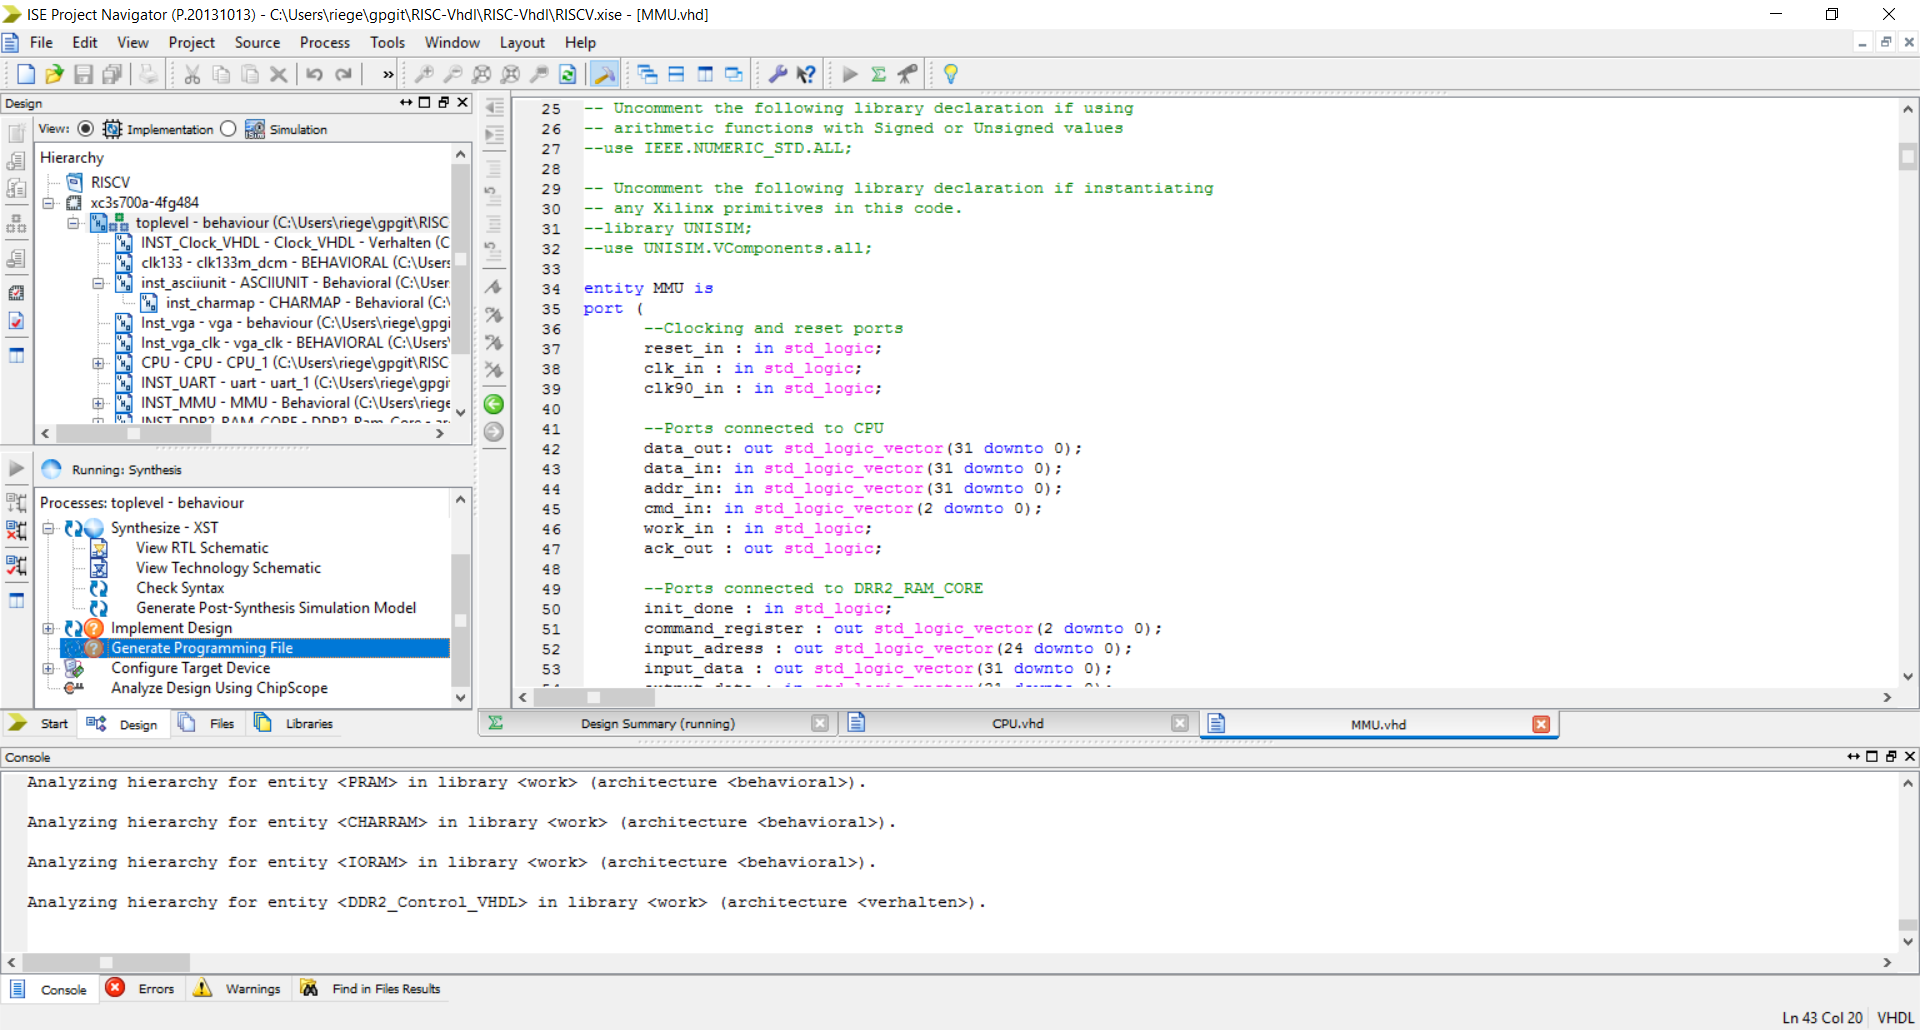
\includegraphics[width=1.0\textwidth]{ISE.png}
\caption{Der Xilinx \textit{ISE Project Navigator}}
\end{figure}

Mittels des Tools \textit{impact}, welches ebenfalls vom Anbieter der
Entwicklungsumgebung Xilinx stammt, konnte in Kombination mit einem
\textit{Cable-Server} das Board \"uber USB gem\"a{\ss} den erstellten
Programming-Files beschrieben werden. Zur Versionsverwaltung wurde dabei
auf ein \textit{Git-Repository} gesetzt.

Um die doch recht umfassende Arbeit des Assemblierens eines Programms nicht
h\"andisch erledigen zu m\"ussen, wurde, wie sp\"ater genauer erl\"autert wird,
ein automatischer Assemblierer in der Skriptsprache Python entwickelt. Da die
Generierung eines Programming-Files und das anschlie\ss{}ende Beschreiben des
FPGAs nichtsdestotrotz jedes Mal mehrere Minuten in Anspruch nahm,
wurden entsprechende Simulatoren verwendet. Zur Verifikation des VHDL-Codes
wurde beispielsweise das Tool \textit{GHDL} in Kombination mit \textit{GTKWave}
benutzt. Auch zum Testen der Assemblerprogramme erfolgte durch einen eigens entworfenen und programmierten Python-basierten Simulator, der die Umgebung des Boards ad\"aquat emuliert.

\newpage


\Chapter{Das Leitwerk}
\label{ch:cu}

\Section{\"Uberblick}
Das Leitwerk \textit{CU} stellt die zentrale Steuereinheit des Prozessors dar und
verwaltet als diese den Program-Counter~(PC) und das Instruction-Register~(IR). Es
interpretiert die Befehle und \"uberwacht ihre Ausf\"uhrung durch ALU und MMU, wobei
der Fokus mehr auf Robustheit und weniger auf Aspekten der
Performanz lag.

Es besitzt f\"ur jeden Befehl eine eigene Zustandsmaschine, deren Verhalten 
durch den Inhalt des Instruction-Registers gesteuert wird. Daher muss jeder
Befehl als letztes das IR mit dem Opcode des folgenden Befehl laden, was dann
in jedem Befehl einzeln optimiert werden kann.

Um den Implementierungsaufwand bei \"Anderungen von Befehlen zu minimieren
wurde ein Compiler-Skript erstellt das mehrere Makros bereitstellt, aus denen
dann die Befehle zusammengebaut werden k\"onnen. Das Skript kompiliert dann
eine Eingabe aus diesen Makros in VHDL-Code.

\Subsection{Legende}
Da jeder Befehl eine eigene Zustandsmaschine besitzt, wird hier f\"ur jeden
Befehl ein eigenes Zustands\-\"uber\-gangs\-dia\-gramm gezeigt. Die Pr\"afixe
``MMU:'' und ``ALU:'' werden genutzt, um anzuzeigen, dass eine Operation an die
jeweiligen Einheit delegiert wird und das Leitwerk lediglich eine Anfrage an
die entsprechende Komponente sendet.

Obwohl in der ISA regelm\"a\ss{}ig verlangt wird, dass Operanden sign-extended
werden, wurde dies in den Zustands\-\"uber\-gangs\-dia\-grammen der \"Ubersicht
halber weggelassen. Im Prozessor ist es selbstverst\"andlich wie in der ISA
beschrieben implementiert.

\Section{Integer Rechenbefehle}
Der Prozessor wurde auf die in \textit{RV32I} und \textit{RV32M} definierten Rechenbefehle
optimiert. Dadurch k\"onnen diese RISC-typischen Befehle sehr schnell
ausgef\"uhrt werden.

\Statemachine{./cu/img/integer_rechenbefehle.pdf}{
Zu\-stands\-\"uber\-gangs\-dia\-gramm der Befehle \Instr{AND[I]},
\Instr{OR[I]}, \Instr{XOR[I]}, \Instr{SLL[I]}, \Instr{SRL[I]}, \Instr{SRA[I]},
\Instr{ADD[I]}, \Instr{SUB}, \Instr{SLT[I][U]}, \Instr{MUL} und
\Instr{MULH[[S]U]}.}{\(op2\) ist entweder das Register, das mit \Ipart{rs2}
angegeben ist, oder eine Immediate (\Ipart{imm}). ``\(\circ\)'' repr\"asentiert
die jeweilige Operation (\(+\), \(-\), \dots{}).
}

\Subsection{Division und Modulo}
Da bei der Division unm\"oglich zu garantieren ist, dass diese immer innerhalb
von drei Takten erfolgreich beendet wird, muss das Leitwerk hier auf eine
Best\"atigung der ALU(\ref{ch:alu}) warten. Diese sieht vor, dass das Rechenwerk
die Leitungen \Vhdl{alu\_data\_in} auf 0 setzt.

\Statemachine{./cu/img/division.pdf}{
Zustands\"ubergangsdiagramm der Befehle \Instr{DIV[U]} und \Instr{REM[U]}.
}{``\(\circ\)'' repr\"asentiert die jeweilige Operation (\(/\), \(\bmod\),
\dots{}).}

\Section{LUI und AUPIC}
Da durch die Integer Rechenbefehle keine 32-Bit Immediates direkt geladen werden
k\"onnen, definiert die \textit{RISC-V-ISA} die Befehle \Instr{LUI} und \Instr{AUPIC}, die
diesen Mangel beheben.

\Statemachine{./cu/img/lui_und_aupic.pdf}{
Zustands\"ubergangsdiagramm der Befehle \Instr{LUI} und \Instr{AUPIC}.
}{\(op2\) ist entweder 0 (bei \Instr{LUI}) oder der aktuelle Program-Counter
(bei \Instr{AUPIC}).}


\Section{Bedingte Spr\"unge}
Da bei Speicherzugriffen auf den DDR2-SDRAM Block der MMU(\ref{ch:mmu}) nicht
garantiert werden kann, dass ein Speicherzugriff ohne Zeit- und Datenverlust
abgebrochen werden kann, wurde auf Branch-Prediction g\"anzlich verzichtet.
Dadurch geh\"oren die bedingten Spr\"unge im Hinblick auf Rechenzeit zu den
teuersten Befehlen des Prozessors.

\Statemachine{./cu/img/beq_und_bgeu.pdf}{
Zustands\"ubergangsdiagramm der Befehle \Instr{BEQ} und \Instr{BGE[U]}.}
{``\(\circ\)'' ist bei \Instr{BEQ} ``\(-\)'', bei \Instr{BGE} die SLT-Operation
und bei \Instr{BGEU} die SLTU-Operation.
}

\Statemachine{./cu/img/bne_und_bltu.pdf}{
Zustands\"ubergangsdiagramm der Befehle \Instr{BNE} und \Instr{BLT[U]}.}
{``\(\circ\)'' ist bei \Instr{BNE} ``\(-\)'', bei \Instr{BLT} die SLT-Operation
und bei \Instr{BLTU} die SLTU-Operation.
}

\Section{Unbedingte Spr\"unge}
Anders als bei bedingten Spr\"ungen, kann bei unbedingten Spr\"ungen das
Sprungzeil immer vorhergesagt werden. Dadurch kann das Schreiben der
Return-Adresse und das Holen des n\"achsten Befehls parallelisiert werden, was
zu einer merklichen Geschwindigkeitssteigerung f\"uhrt.

\Statemachine{./cu/img/unbedingte_spruenge.pdf}{
Zustands\"ubergangsdiagramm der Befehle \Instr{JAL} und \Instr{JALR}.}
{\(op2\) ist bei \Instr{JAL} der Program-Counter und bei \Instr{JALR} das
Register, welches durch \Ipart{rs1} adressiert wird.
}

\Section{LOAD}
Der LOAD-Befehl l\"adt aus dem Speicher immer einen 32-Bit Wert, den das
Leitwerk dann zuschneidet. Dies sollte urspr\"unglich die Implementierung der
MMU vereinfachen und aligned-Speicherzugriffe beschleunigen. Es hat sich
allerdings im Projektverlauf ein nachteiliger Charakter in dieser Entscheidung offenbart, da die Ausf\"uhrungsdauer des Befehls in der Praxis
haupts\"achlich von der adressierten Speicherkomponente bestimmt wird.

\Statemachine{./cu/img/load.pdf}{
Zustands\"ubergangsdiagramm der Befehle \Instr{LB[U]}, \Instr{LH[U]} und
\Instr{LW}.}{\(width\) ist je nach Befehl 1,~2~oder~4.
}

\Section{STORE}
Der Store-Befehl ist mit nur einem Rechen- und Speicherwerk nicht zu
parallelisieren, was dazu f\"uhrt, dass er den langsamsten Befehl des
Leitwerks darstellt. Da Schreibzugriffe jedoch generell auf RISC-Architekturen
sehr hohe Kosten hinsichtlich der ben\"otigten Rechenzeit aufweisen, sind
Compiler und Programmierer ohnehin dazu angehalten, schreibende
Speicherzugriffe m\"oglichst zu vermeiden.

\Statemachine{./cu/img/store.pdf}{
Zustands\"ubergangsdiagramm des Befehle \Instr{SB}, \Instr{SH} und \Instr{SW}.}
{\(width\) ist je nach Befehl 1, 2 oder 4.
}

\Section{Timer und Counter}
Wie in der RISC-V-ISA gefordert existiert des Weiteren ein Counter, der die
Anzahl der bisher ausgef\"uhrten Befehle z\"ahlt. Au\ss{}erdem gibt es einen
Timer, der analog dazu die Anzahl der bereits vergangenen Takte speichert. Da
das Entwicklungsboard allerdings keine Echtzeituhr bereitstellt, greift die
Implementierung dieser Funktionalit\"at auf den Taktz\"ahler zur\"uck.

Ausgelesen werden k\"onnen diese Counter durch die Befehle
\Instr{RDINSTRET[H]}\nolinebreak{}, \Instr{RDCYCLE[H]} und \Instr{RDTIME[H]}.

\Statemachine{./cu/img/timer_und_counter.pdf}{
Zustands\"ubergangsdiagramm der Befehle \Instr{RDINSTRET[H]},
\Instr{RDCYCLE[H]} und \Instr{RDTIME[H]}.}{\(counter\) sind die oberen bzw.
unteren 32 Bit des jeweiligen 64-Bit-Z\"ahlers.
}

\newpage

\Chapter{Die arithmetisch-logische Einheit}
\label{ch:alu}

Die arithmetisch-logische Einheit \textit{ALU} ist verantwortlich f\"ur die Durchf\"uhrung aller f\"ur die Befehlsausf\"uhrung durch das Leitwerk relevanten Rechenoperationen. Zus\"atzlich verwaltet sie die Register des Prozessors.


\Section{\"Uberblick}
Zentrale Design-Idee hinter der ALU ist es, mehr als einen reinen Multiplexer f\"ur Befehle zu entwickeln. Stattdessen bietet sie dem Leitwerk ein Interface,
\"uber das Operationen auf Registern oder Immediates angefragt werden k\"onnen. Hierzu wurde eine Menge von Prozessor-internen Opcodes definiert.

Da die ALU auch zur Ausf\"uhrung von nicht-arithmetischen Maschinenbefehlen, beispielsweise bei Spr\"ungen, oft beansprucht wird, sollte der Synchronisations- und Kommunikationsaufwand zwischen ALU und Leitwerk m\"oglichst reduziert werden.
Aus diesem Grund werden grunds\"atzlich alle Befehle (exklusive der Division) mittels einer Zustandsmaschine innerhalb von drei Takten ausgef\"uhrt, wodurch kein Synchronisations-Protokoll zwischen ALU und Leitwerk von N\"oten ist.

Um die Komplexit\"at des Leitwerks zu reduzieren, wurde die Low-Level-Verwaltung der Register in die ALU ausgelagert. Diese wurden als Dual-Port-Blockram realisiert, um die Anzahl an belegten Slices auf dem FPGA zu reduzieren.

\Section{Das Interface}
\begin{figure}[H]
	\centering
	\label{fig:aluinterface}
		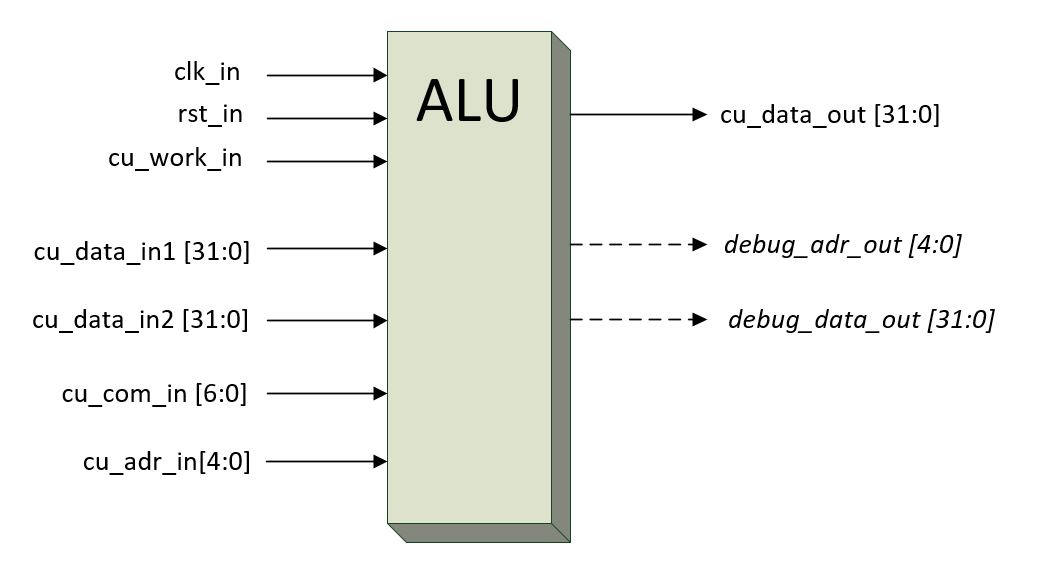
\includegraphics[width=0.7\textwidth]{interface.jpg}
	\caption[Schnittstelle der ALU-Einheit]{Schnittstelle der ALU mit Portnamen und -breiten}
\end{figure}

Neben zwei 32-Bit-Eing\"angen f\"ur Operanden, gibt es einen dedizierten Eingang f\"ur Registeradressen sowie einen zur Auswahl der gew\"unschten Operation. 
Der Adresseingang dient hierbei lediglich zur Adressierung des Zielregisters. Da alle Befehle nur aus zwei Operanden bestehen, werden die Operanden-Eing\"ange entweder zur \"Ubermittlung von Immediates, oder zur Adressierung der Operanden-Register verwendet, was die Anzahl der Eing\"ange reduziert.

Aktiviert wird die ALU vom Leitwerk \"uber \Vhdl{cu\_work\_in} und innerhalb von drei Takten liegt dann auf \Vhdl{cu\_data\_out} das entsprechende Ergebnis an.

\Section{Interne Befehle}
Zur Auswahl der gew\"unschten Operation bietet die ALU einen 7 Bit breiten Befehls-Eingang an.
Jeder Befehl besteht dabei aus drei Sektionen\vspace{10pt}:

\Instr{Reg1 | Reg2 | OpC}\vspace{5pt}

Das oberste Bit \Ipart{Reg1} entscheidet dar\"uber, ob der erste Operand als Immediate vom Dateneingang \Vhdl{cu\_data\_in1}, oder aus dem durch \Vhdl{cu\_data\_in1} adressierten Register genommen wird.
Analog wird anhand \Ipart{Reg2} determiniert, ob auf \Vhdl{cu\_data\_in2} eine Adresse oder ein Immediate anliegt.
Darauf folgt der f\"unf Bit umfassende interne OpCode. Zur Verf\"ugung stehen OpCodes f\"ur:

\begin{itemize}
\item Addition, Subtraktion
\item Logische Shifts
\item Arithmetische Shifts
\item Set Less Than Immediate Signed und Unsigned (SLT,SLTU)
\item Multiply Lower auf Signed und Unsigned-Operanden
\item Multiply Upper auf Signed und Unsigned Operanden
\item Division Signed und Unsigned
\item Modulo-Rechnung Signed und Unsigned
\end{itemize}

\Section{Befehlsausf\"uhrung}


\Statemachine{./alu/img/states.pdf}{
Zustands\"ubergangsdiagramm der Befehlsausf\"uhrung innerhalb der ALU
}{}

Die Ausf\"uhrung von Befehlen ist \"uber eine State-Machine mit drei zentralen Zust\"anden, sowie zwei Zusatzzust\"anden f\"ur Signed- und Unsigned-Division bzw. Modulo-Operationen realisiert. In jedem der drei zentralen Zust\"ande wird dabei nur f\"ur einen Takt verblieben.


\Subsection{State 1 - Selektion der Operanden}
Die ALU wartet in State 1, bis vom Leitwerk das entsprechende Work-Signal gesendet wird.
Anschlie\ss{}end werden auf Grundlage des oben beschriebenen Befehls zwei Operanden-Signale \Vhdl{s\_op1} und \Vhdl{s\_op2} mit einer Immediate vom Daten-Eingang belegt, oder aber es wird ein Register-Lesezugriff angesto"sen, dessen Ergebnis dann im n\"achsten Takt zur Verf\"ugung steht.


\Subsection{State 2 - Operationsausf\"uhrung}
State 2 dient der eigentlichen Befehlsausf\"uhrung. Realisiert ist er als Case-Statement \"uber den internen OpCode. Innerhalb jedes Cases wird zwischen den vier m\"oglichen Kombinationen auf Immediate- und Register-Operanden unterschieden.
Dies ist n\"otig, da das Ergebnis eines m\"oglichen Register-Zugriffs erst in diesem Takt anliegt und deshalb nicht einfach die \Vhdl{s\_op1}- und \Vhdl{s\_op2}-Signale f\"ur Immediate-Operationen \"uberschrieben werden k\"onnen.
Die Operation wird auf den jeweiligen Operanden durchgef\"uhrt und in einem Akkumulator gespeichert.\vspace{10pt}


Ein Gro"steil der Operationen ist \"uber die \Vhdl{IEEE.NUMERIC\_STD.ALL} Operatoren realisiert und kann innerhalb dieses einen Taktes vollst\"andig abgeschlossen werden.

Da die Standard-Multiplikation von 32-Bit-Werten zu einem 64 Bit langen Ergebnis f\"uhrt, werden Multiplikationsergebnisse nicht im normalen Akkumulator-Signal \Vhdl{acc}, sondern im Zusatzsignal \Vhdl{mult-result} gespeichert. Der VHDL-Compiler erlaubte es nicht, unmittelbar auf das Ergebnis zuzugreifen und entweder die oberen oder unteren 32 Bit in \Vhdl{acc} zu speichern.\vspace{10pt}

Da der Standard-Operator \Vhdl{sar} nicht durch die gegebene Entwicklungsumgebung synthetisierbar ist, wird bei einem arithmetischen Rechtsshift um {n} Stellen zus\"atzlich das oberste Bit des ersten Operanden zwischengespeichert, um im nachfolgenden State, wenn n\"otig, die oberen {n} Bits auf {1} zu setzen.\vspace{10pt}

Im Falle einer Modulo- oder Unsigned-Division wird in State 2 der \"Ubergang in State 4 bzw. 5 eingeleitet. Ansonsten erfolgt ein direkter \"Ubergang in State 3.

\Subsection{State 3 - Write-Back}
In State 3 werden die akkumulierten Ergebnisse in das von der ALU adressierte Register geschrieben.

Bei den meisten der Operationen kann dies unmittelbar erfolgen. Bei Multiplikationsoperationen allerdings muss jedoch zuerst anhand des OpCodes entschieden werden, ob die oberen oder unteren 32 Bit des Ergebnisses gespeichert werden sollen. Abh\"angig vom Status-Bit f\"ur arithmetische Shifts um {n} Stellen werden, wie oben beschrieben, gegebenenfalls die oberen n Bits des Ergebnisses auf {1} gesetzt.\vspace{10pt}


Neben dem Speichern des Ergebnisses werden zwei zus\"atzliche Ausg\"ange belegt:

Auf \Vhdl{cu\_data\_out} wird das Ergebnis angelegt. Einzige Ausnahme stellt die Division bzw. Modulorechnung dar, bei der als Synchronisationssignal der Daten-Ausgang mit 0 belegt wird. Das ist n\"otig, da die Division vom normalen 3-Takte-Schema abweicht.
Auch die Debug-Schnittstelle erh\"alt \"uber \Vhdl{debug\_data\_out} den entsprechenden Wert sowie das relevante Register \"uber \Vhdl{debug\_adr\_out}.

\Subsection{State 4 - Division Unsigned}
Um die Anzahl an n\"otigen Takten zu reduzieren, wird bei der Umsetzung der Unsigned Division eine durch den \textit{Core-Generator} erstellte Divisionseinheit genutzt, welche eine gepipelinte Variante der SRT-Division durchf\"uhrt. Obwohl der Prozessor keinen unmittelbaren Nutzen aus dem Pipelining zieht, kann durch die effiziente Implementierung die Anzahl an n\"otigen Takten reduziert werden. Zus\"atzlich liefert die Einheit sowohl den Rest, als auch das Divisionsergebnis, weshalb die beiden Operationen gleich behandelt werden k\"onnen.


Hierzu werden bei Betreten des States die Operanden angelegt. Danach wird mit einem Z\"ahler gewartet, bis das Ergebnis der Operation anliegt.
Anschlie\ss{}end werden je nach Anfrage entweder der Rest oder das Ergebnis in den Akkumulator eingelesen und in State 3 \"ubergegangen.

\Subsection{State 5 - Division Signed}
Die Implementierung verl\"auft analog zu State 4, abgesehen davon, dass eine Einheit zur Durchf\"uhrung von Signed-Divisionen verwendet wird.

\Section{Die Register}
Insgesamt stellt die ALU 32 Register der Breite 32 Bit bereit, wobei Register x0 konstant mit dem Wert 0 belegt und nicht \"uberschreibbar ist. Dies ist zum Beispiel n\"utzlich beim unver\"anderten Laden eines Registers.

Implementiert wurden die Register als Dual-Port-Blockram. Dieses Vorgehen erm\"oglicht den zeitgleichen Zugriff auf zwei verschiedene Speicherinhalte, was gerade bei Register-Register-Operationen von Vorteil ist. Zus\"atzlich wird dadurch die Anzahl an verwendeten Slices reduziert, da dedizierte Blockram-Bausteine logisch zum Registersatz zusammengef\"ugt werden.\vspace{10pt}

Die Umsetzung erfolgte dabei nicht \"uber eine Variante aus dem \textit{Core-Generator}, sondern durch die Einhaltung eines speziellen Verwendungsprotokolls, sodass der Compiler das definierte \textit{std\_logic\_vector}-Array automatisch in einen Blockram umsetzt.

Voraussetzung daf\"ur ist, dass nicht direkt auf Register-Inhalten operiert wird, sondern sie zuerst in einem Signal zwischengespeichert und im n\"achsten Takt verwendet werden. Dies ist aber ohnehin durch die 3-stufige State-Machine der ALU garantiert.

\Section{Reset}
Die ALU verf\"ugt zudem \"uber einen Reset-Eingang, welcher direkt von der Toplevel-Komponente weitergeleitet wird. Bei einem Reset wird das Rechenwerk in den State 0 \"uberf\"uhrt, um nach Ende des Resets wieder Befehle des Leitwerks entgegennehmen zu k\"onnen.

Zus\"atzlich wird der Divisions-Flankenz\"ahler auf Null gesetzt, um keine Fehler bei nachfolgenden Operationen zu versursachen. Das Reset-Signal wird auch an den Reset (SCLR)-Eingang der Divisionseinheit weitergeleitet.

Ein Reset der Register erfolgt nicht, sodass abgesehen vom Register x0 f\"ur den Entwickler eines Nutzerprogramms keine Aussage \"uber die initialen Werte der Register m\"oglich ist.

\newpage

\Chapter{Die MMU}
\label{ch:mmu}

Die MMU (Memory Management Unit) verwaltet den in Bl\"ocke gegliederten Speicherbereich und die darauf erfolgenden Zugriffe. Die Einheit bietet dabei eine Schnittstelle f\"ur lesende und schreibende Speicheranfragen, welche in unterschiedlichen Zeitintervallen bearbeitet werden.

\Section{\"Uberblick}

Der adressierbare Speicher innerhalb des Prozessors ist blockweise organisiert. Die MMU verwaltet einerseits die einzelnen Controller f\"ur die jeweiligen RAM-Bl\"ocke und taktet andererseits die angefragten Zugriffe auf diese.

Sie ist aufgrund der \"uberwiegend sehr \"ahnlichen Adressierungsprozeduren intern durch eine Statemachine realisiert, welche anhand einer Speicheradresse die jeweiligen Speicheranfragen an den dem RAM-Block entsprechenden Controller weiterleitet.

Um eine reibungslose Kommunikation mit diesen Controllern zu gew\"ahrleisten, ist die MMU mit einer vom restlichen Prozessor unterschiedlichen Frequenz, 133 MHz, getaktet. Dies ist vor allem mit dem integrierten DDR2-SDRAM\footnote{Genauer handelt es sich um einen Micron Technology DDR2-SDRAM (MT47H32M1)}, welcher mit eben diesem Takt versorgt werden muss, um Daten halten zu k\"onnen, begr\"undet: Die Tatsache, dass die Integration dieser Komponente besonders zeitaufw\"andig verlief, rechtfertigt diese Designentscheidung. Daraus resultieren zus\"atzlich ben\"otigte Synchronisations- und Kommunkationsmechanismen mit dem \"ubergeordneten Leitwerk.

\Section{Interface}
Das Interface der MMU untergliedert sich haupts\"achlich in drei verschiedene Komponenten: Einerseits Signale zur Kommunikation mit dem Leitwerk, andererseits durch das Toplevel-Modul nach oben geleitete Signale zur Adressierung des DDR2-SDRAMs, welche vom in der MMU verwalteten Controller generiert werden, und zuletzt nach oben geleitete Daten- und Adressleitungen, die die ASCII-Einheit konstant mit Daten versorgt.

\begin{figure}[H]
	\label{fig:mmuinterface}
	\centering
		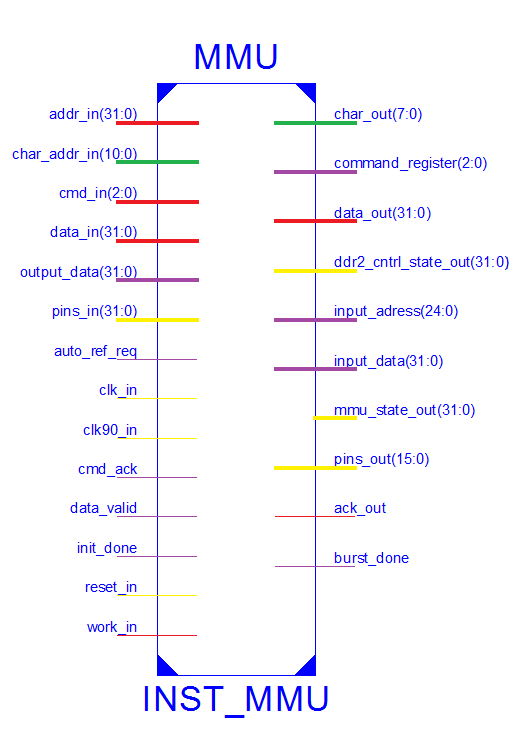
\includegraphics[width=0.5\textwidth]{interface.png}
	\caption[Schnittstelle der MMU-Einheit]{Schnittstelle der MMU-Einheit, Signale farblich gruppiert: \textit{Rot} = Kommunikation mit Leitwerk, \textit{Gr\"un} = Character-Ausgabe an ASCII-Einheit, \textit{Violett} = Verbindung mit DDR2-SDRAM, \textit{Gelb} = Sonstige}
\end{figure}

\Subsection{Kommunikation mit dem Leitwerk}

Die Kommunikation mit dem Leitwerk l\"asst sich im Wesentlichen in Daten-, Adress- und Synchronisationsleitungen untergliedern. Dabei sendet das Leitwerk \"uber das Signal \Vhdl{cmd\_in} die angefragte Operation. Die MMU reagiert allerdings erst auf ein Setzen des \Vhdl{work\_in} Signals mit der Bearbeitung der Anfrage. Der 3-Bit-Vektor \Vhdl{cmd\_in} ist wie folgt aufgebaut:

\begin{table}[H]
	\begin{center}
	\begin{tabular}{| l | l |}
		\hline
		Bit 2 & Bit 1 - 0 \\ \hline
		0 := Read, 1 := Write & 0 := 8 Bit, 1 := 16 Bit, 3 := 32 Bit \\ 		\hline
	\end{tabular}
	\caption{Aufbau des Kommunikationssignals zwischen Leitwerk und MMU}
\end{center}
\end{table}

Als Ausgabe liefert die MMU dem Leitwerk ein Acknowledgement \Vhdl{ack\_out}, welches signalisiert, dass die MMU bereit ist, eine neue Anfrage zu bearbeiten und indirekt damit auch Auskunft dar\"uber gibt, ob die bereits gesendete Anfrage erfolgreich bearbeitet wurde. Im Falle eines lesenden Speicherzugriffs wird, sofern das Acknowledgement-Signal den Wert 1 angenommen hat, gew\"ahrleistet, dass der Datenausgang \Vhdl{data\_out} korrekt belegt wurde.

Es sei angemerkt, dass im Zuge der Entwicklung und aufgrund der stark \"uberwiegenden Zahl der 32-Bit Lesezugriffe (vor allem im Zuge des Ladens eines Befehls) beschlossen wurde, dass jeder lesende Speicherzugriff ungeachtet der im \Vhdl{cmd\_in} definierten Datenbreite 32-Bit liest. Theoretisch bietet die MMU allerdings auch die M\"oglichkeit, 8-Bit oder 16-Bit Lesezugriffe durchzuf\"uhren.

\Subsection{Durch die MMU geleitete Signale an andere Komponenten}

Wie eingangs erw\"ahnt lassen sich die \"ubrigen Signale dem Weiterleiten von Signalen aus einerseits dem Controller der DDR2-SDRAM-Komponente sowie den kontinuierlichen lesenden Anfragen der ASCII-Einheit an den entsprechenden CHARRAM-Block (die parallel und unabh\"angig von der Funktionalit\"at der MMU laufen) zuordnen und werden hier nicht weiter vertieft.

\Section{Aufbau des Speichers}

Wie bereits geschildert, wird der Speicher in verschiedene Bereiche unterschiedlicher Gr\"o\ss{}e untergliedert. Jeder dieser Bereiche wird von einem Controller verwaltet, welcher bei einer eingehenden Anfrage durch die MMU angesprochen wird. Dabei h\"angt die Bearbeitungsdauer ma\ss{}geblich vom adressierten Speicherblock ab.

Aus der durch den Prozessor implementierten Wortgr\"o\ss{}e von 32 Bit ergibt sich ein Adressraum, der potenziell $2^{32}$ Speicherzellen mit einer Gr\"o\ss{}e von je 8 Bit umfasst. Dass nicht jeder dadurch zur Verf\"ugung stehende Bereich auch tats\"achlich auch nutzbar ist, l\"asst sich auf die vom FPGA zur Verf\"ugung gestellten Speicherressourcen zur\"uckf\"uhren.

Stattdessen wird die Adresse in ein Pr\"afix, welches den adressierten Speicherbereich bestimmt, und ein Offset innerhalb dieses Speicherblocks wie folgt unterteilt:

\begin{table}[H]
\begin{center}
	\begin{tabular}{| l | l |}
		\hline
		Bit 31 - 28 & Bit 27 - 0 \\ \hline
		Pr\"afix & Offset \\ \hline
	\end{tabular}
\end{center}
\caption{Aufbau des Adressvektors}
\end{table}

Insgesamt existieren f\"unf zul\"assige Werte f\"ur das 4-Bit Pr\"afix, wobei Zugriffe auf nicht g\"ultige Speicherpr\"afixe nicht verarbeitet werden. Zudem unterscheiden sich die Gr\"o\ss{}en der jeweiligen Speicherbl\"ocke von dem potenziell $2^{28}$ Bit gro\ss{}en Raum innerhalb eines Blocks. Aufgrund der Tatsache aber, dass diese sich stets als nat\"urliche Potenz von 2 darstellen lassen, kann durch Spiegelung des tats\"achlich nutzbaren Speicherraums der gesamte vom Offset darstellbare Bereich adressiert werden. Im Endeffekt wird der Offset also lediglich in seiner wirksamen Gr\"o\ss{}e entsprechend des Speicherblocks beschnitten. Die folgende Tabelle zeigt die implementierten Speicherbl\"ocke sowie deren nutzbare Gr\"o\ss{}e.

\begin{table}[H]
	\begin{center}
	\label{tab:ramlayout}
	\begin{tabular}{| l | l | l | l |}
		\hline
		Pr\"afix & K\"urzel & Gr\"o\ss{}e in Bytes & Kurzbeschreibung \\ \hline
		0x0 & BIOS & $2^{11}$ & Programmeinsprungspunkt \\ \hline
		0x1 & SDRAM & $2^{16}$ bzw. $512$ MBit & DDR2-SDRAM\\ \hline
		0x2 & CHARRAM & $2^{11}$ & Character-Anzeige \\ \hline
		0x3 & IORAM & $2^{3}$ & Memory-Mapped I/O \\ \hline
		0x4 & SERIALRAM & $2^{11}$ & Serielle Schnittstelle \\ \hline
	\end{tabular}
	\end{center}
	\caption{Aufbau des Speichers als Bl\"ocke}
\end{table}

Dabei sind alle Bl\"ocke, ausgenommen der DDR2-SDRAM-Block, durch auf dem FPGA ver\-f\"ug\-baren Dual-Port-Block\-ram realisiert, sodass die implementierten Controller im Groben gleich sind. Angemerkt sei an dieser Stelle, dass - in Absprache mit dem Betreuer - der Controller f\"ur den DDR2-SDRAM eine Implementierung von Opencores\footnote{\url{http://opencores.org/project,ddr2_sdram}} verwendet und entsprechend den Anforderungen abge\"andert wurde.

Jeder Speicherbereich wird von der MMU im Little-Endian-Format adressiert, was insbesondere bei 16-Bit beziehungsweise 32-Bit Zugriffen ber\"ucksichtigt werden muss.

\Section{Memory-Mapped I/O}
\label{sec:mmuio}
Einer der geschilderten Speicherbl\"ocke, genauer der IORAM, stellt die Schnittstelle zwischen Benutzer und Programmcode dar. Dabei sind einige der auf dem FPGA verf\"ugbaren Ein- und Ausgabem\"oglichkeiten direkt auf einzelne Bits innerhalb der Speicherzellen des IORAMs gemappt. Aus den acht verf\"ugbaren Speicherzellen sind effektiv sechs nutzbar:

\begin{table}[H]
\begin{center}
	\begin{tabular}{| c | c | c | c | c | c | c | c | c | c |}
	\hline
	Zelle & R/W & Bit 7 & Bit 6 & Bit 5 & Bit 4 & Bit 3 & Bit 2 & Bit 1 & Bit 0 \\ \hline
	0x0 & Read-Only & BTN 0 & - & - & - & - & - & - & - \\ \hline
	0x1 & Read-Only & SW 3 & SW 2 & SW 1 & SW 0 & BTN 4 & BTN 3 & BTN 2 & BTN 1 \\ \hline
	0x2 & Read/Write & LED 7 & LED 6 & LED 5 & LED 4 & LED 3 & LED 2 & LED 1 & LED 0 \\ \hline
	0x3 & Read/Write & - & - & - & - & - & - & - & - \\ \hline
	0x4 & Read-Only & UART 7 & UART 6 & UART 5 & UART 4 & UART 3 & UART 2 & UART 1 & UART 0 \\ \hline
	0x5 & Read-Only & - & - & - & - & - & - & UART & UART \\
	 &  &   &   &   &   &   &   & VALID & ERR \\ \hline
	0x6 & Unused & - & - & - & - & - & - & - & - \\ \hline
	0x7 & Unused & - & - & - & - & - & - & - & - \\ \hline
	\end{tabular}
\end{center}
\caption{Memory-Mapped I/O im Detail}
\end{table}

Dabei steht BTN jeweils f\"ur entsprechende Buttons auf dem Board, SW entspricht einem Schalter und LED den Ausgabe-LEDs. Au\ss{}erdem sind die Eingabedaten der seriellen Schnittstelle in Form eines 8-Bit Vektors sowie einem Best\"atigungssignal, dass dieser vollst\"andig \"ubertragen wurde und einem Fehlersignal, das ebenfalls von der seriellen Schnittstelle ausgeht, ebenfalls auf den IORAM gemappt. Angemerkt sei an dieser Stelle aber, dass der Prozessor nicht konsistent schnell genug arbeitet\footnote{Die h\"aufige Synchronisation mit dem DDR2-SDRAM Block verursacht nichtdeterministisch auftretende Abweichungen im Bezug auf Speicherzugriffszeiten}, um diese Funktionalit\"at wirklich sinnvoll zu nutzen, weswegen zur Initialisierung des Programmspeichers auch eine andere Methode verwendet wird. Bits, die nicht genutzt und in der Tabelle mit `-' vermerkt sind, entsprechen stets dem konstanten Wert 0 und bieten daher auch keinerlei Speicherf\"ahigkeit.

Die nachfolgende Abbildung~\ref{fig:pinning} zeigt, wo sich welches Ein-/Ausgabesignal auf der Hardware wiederfindet. Dabei entsprechen die Bezeichner denen aus der zuvor abgebildeten Tabelle.

\begin{figure}[H]
	\centering
	\label{fig:pinning}
		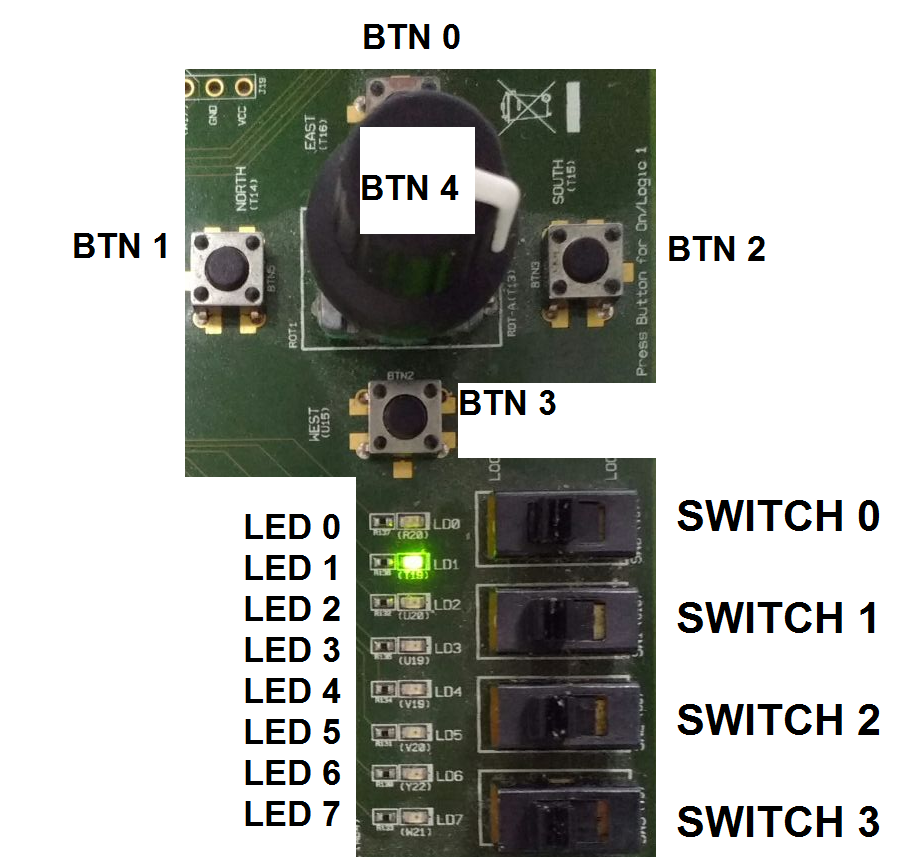
\includegraphics[width=0.5\textwidth]{pinning.png}
	\caption{Verteilung der I/O-Signale}
\end{figure}


\Section{Implementierung als State Machine}

Aufgrund der identisch aufgebauten Controller f\"ur die meisten Speicherbl\"ocke ist die MMU durch eine State Machine realisiert. Dabei die MMU zwar im State MMU-IDLE initialisiert, wechselt bei einem Reset den Zustand aber sofort zu MMU-RESET.

Das nachfolgende Zustands\"ubergangsdiagramm veranschaulicht die durch einen Lese- oder Schreibzugriff entstehende Prozedur.

\Statemachine{./mmu/mmu_state.pdf}{
Zustands\"ubergangsdiagramm der MMU.}
{\"Uberg\"ange zum Zustand \textbf{MMU-RESET}, die von jedem anderen Zustand durch \Vhdl{rst\_in = '1'} ausgel\"ost werden, sind der \"Ubersicht halber ausgelassen.}

\Subsection{MMU-IDLE}

Im Zustand MMU-IDLE wartet die Einheit auf das Eingehen eines Befehls \"uber das \Vhdl{cmd\_in} Signal. Solange dies nicht erfolgt, wird das Synchronisationssignal \Vhdl{ack\_out} mit dem Wert 1 belegt. Anderenfalls wird die Eingabeadresse ausgewertet, die durchzuf\"uhrende Operation an den entsprechenden RAM-Controller weitergeleitet und die Einheit in den Zustand MMU-WAITING \"uberf\"uhrt.

\Subsection{MMU-WAITING}

Durch diesen Zustand wird die Ausf\"uhrung eines Lese- oder Schreibzugriffs solange verz\"ogert, bis der entsprechende RAM-Controller die 8-Bit Anfrage erfolgreich bearbeitet hat. Im Fall des DDR2-SDRAM-Controllers erfolgt dies \"uber ein Synchronisationssignal, anderenfalls kann mit einer festen Wartedauer von einem Takt gerechnet werden. W\"ahrend des Wartevorgangs werden die Befehle, die am entsprechenden RAM-Controller anliegen, entfernt.

Sollte der Controller bereit sein, eine neue 8-Bit Anfrage zu verarbeiten, wird die MMU in den Zustand MMU-DATA-VALID \"uberf\"uhrt.

\Subsection{MMU-DATA-VALID}
In diesem Zustand werden, sofern es sich bei der zuletzt durchgef\"uhrten Operation um einen Lesezugriff gehandelt hat, die gelesenen Daten mittels eines Buffer-Signals zwischengespeichert. Au\ss{}erdem wird die Einheit je nach Zugriffsmodus in den Zustand MMU-READ-NEXT beziehungsweise MMU-WRITE-NEXT \"uberf\"uhrt.

\Subsection{MMU-READ-NEXT}

Sofern noch weitere 8-Bit Zellen gelesen werden m\"ussen, wird eine neue lesende Anfrage an den entsprechenden RAM-Controller weitergeleitet und  die Einheit wieder in den Zustand MMU-WAITING \"uberf\"uhrt. Anderenfalls wechselt die MMU in den Zustand MMU-READ-DONE.

\Subsection{MMU-READ-DONE}

Alle gelesenen und zwischengespeicherten Daten werden gem\"a\ss{} dem Little-Endian-Encoding zusammengesetzt und auf der Datenausgabeleitung an das Leitwerk \"ubergeben. Damit einher geht das Setzen des Acknowledgements-Signals \Vhdl{ack\_out} auf den Wert 1 sowie der Zustandswechsel nach MMU-IDLE.

\Subsection{MMU-WRITE-NEXT}

Sollte der vom Leitwerk geforderte Schreibzugriff weitere schreibende 8-Bit Zugriffe erfordern, wird in diesem Zustand der der Adresse entsprechende RAM-Controller mit neuen Daten und einer inkrementierten Adresse angesprochen und die MMU-Einheit in den Zustand MMU-WAITING \"uberf\"uhrt. Anderenfalls wechselt die MMU in den Zustand MMU-WRITE-DONE.

\Subsection{MMU-WRITE-DONE}

Da nach einem erfolgreichen Schreibzugriff keinerlei Ausgabedaten \"ubermittelt werden m\"ussen, wird in diesem Zustand lediglich das Acknowledgement-Signals \Vhdl{ack\_out} auf den Wert 1 gesetzt sowie die Einheit zur\"uck in den Zustand MMU-IDLE \"uberf\"uhrt.

\Subsection{MMU-RESET}

Bei einem Reset wechselt die MMU ungeachtet ihres derzeitigen Zustands in den MMU-RESET Zustand und unterbricht alle derzeitigen Anfragen ausnahmslos. Da die Einheit das eingehende Reset-Signal an alle RAM-Controller weitergeleitet, wird in diesem Zustand lediglich auf  die Beendigung der Resets jedes einzelnen Controllers gewartet. Sollten diese wieder bereit f\"ur neue Anfragen sein, wechselt die MMU wieder in den MMU-IDLE Zustand.

\Section{Zugrifssdauer}

Aus dem geschilderten detaillierten Ablauf eines Zugriffs innerhalb der MMU lassen sich nun f\"ur die einzelnen Speicherbl\"ocke die exakten Zugriffsdauern beziehungsweise im Fall des DDR2-SDRAMs, welcher unter Umst\"anden durch einen periodisch auftretenden Auto-Refresh eine erh\"ohte Zugriffszeit ben\"ontigt, eine Mindestzugriffsdauer errechnen.

\begin{table}[H]
\begin{center}
	\begin{tabular}{| l | l | l | l |}
		\hline
		Datengr\"o\ss{}e & (minimale) Zugriffsdauer \\ \hline
		8-Bit & 4 Takte \\ \hline 
		16-Bit & 7 Takte \\ \hline
		32-Bit & 13 Takte \\ \hline
	\end{tabular}
\end{center}
\caption{Zugriffsdauer einzelner Speicherzugriffe}
\end{table}

Aufgrund der identischen Struktur der RAM-Controller f\"ur als Dual-Port-Blockram realisierte Speicherbereiche ergeben sich f\"ur jene Speicherbl\"ocke identische Zugriffszeiten sowohl f\"ur lesende und schreibende Zugriffe, wobei eine 8-Bit Anfrage immer genau einen Takt kostet. Da der DDR2-SDRAM f\"ur seine Zugriffsdauer im Bezug auf lesende und schreibende Operationen nicht nach oben hin abgesch\"atzt werden kann, jedoch keinesfalls weniger als einen Takt brauchen wird, entsprechen die Mindestzugriffszeiten ebenfalls der oben dargestellten Tabelle.

\newpage


\Chapter{Die ASCII-Unit}

\label{ch:asciiunit}
Die ASCII-Unit stellt die grafische Schnittstelle zwischen Prozessor und Benutzer dar, und fungiert somit als Hauptinterface, die implementierte Funktionalit\"at auf dem Monitor darzustellen.

\begin{figure}[!htbp]
	\centering
	\label{fig:exampletext}
	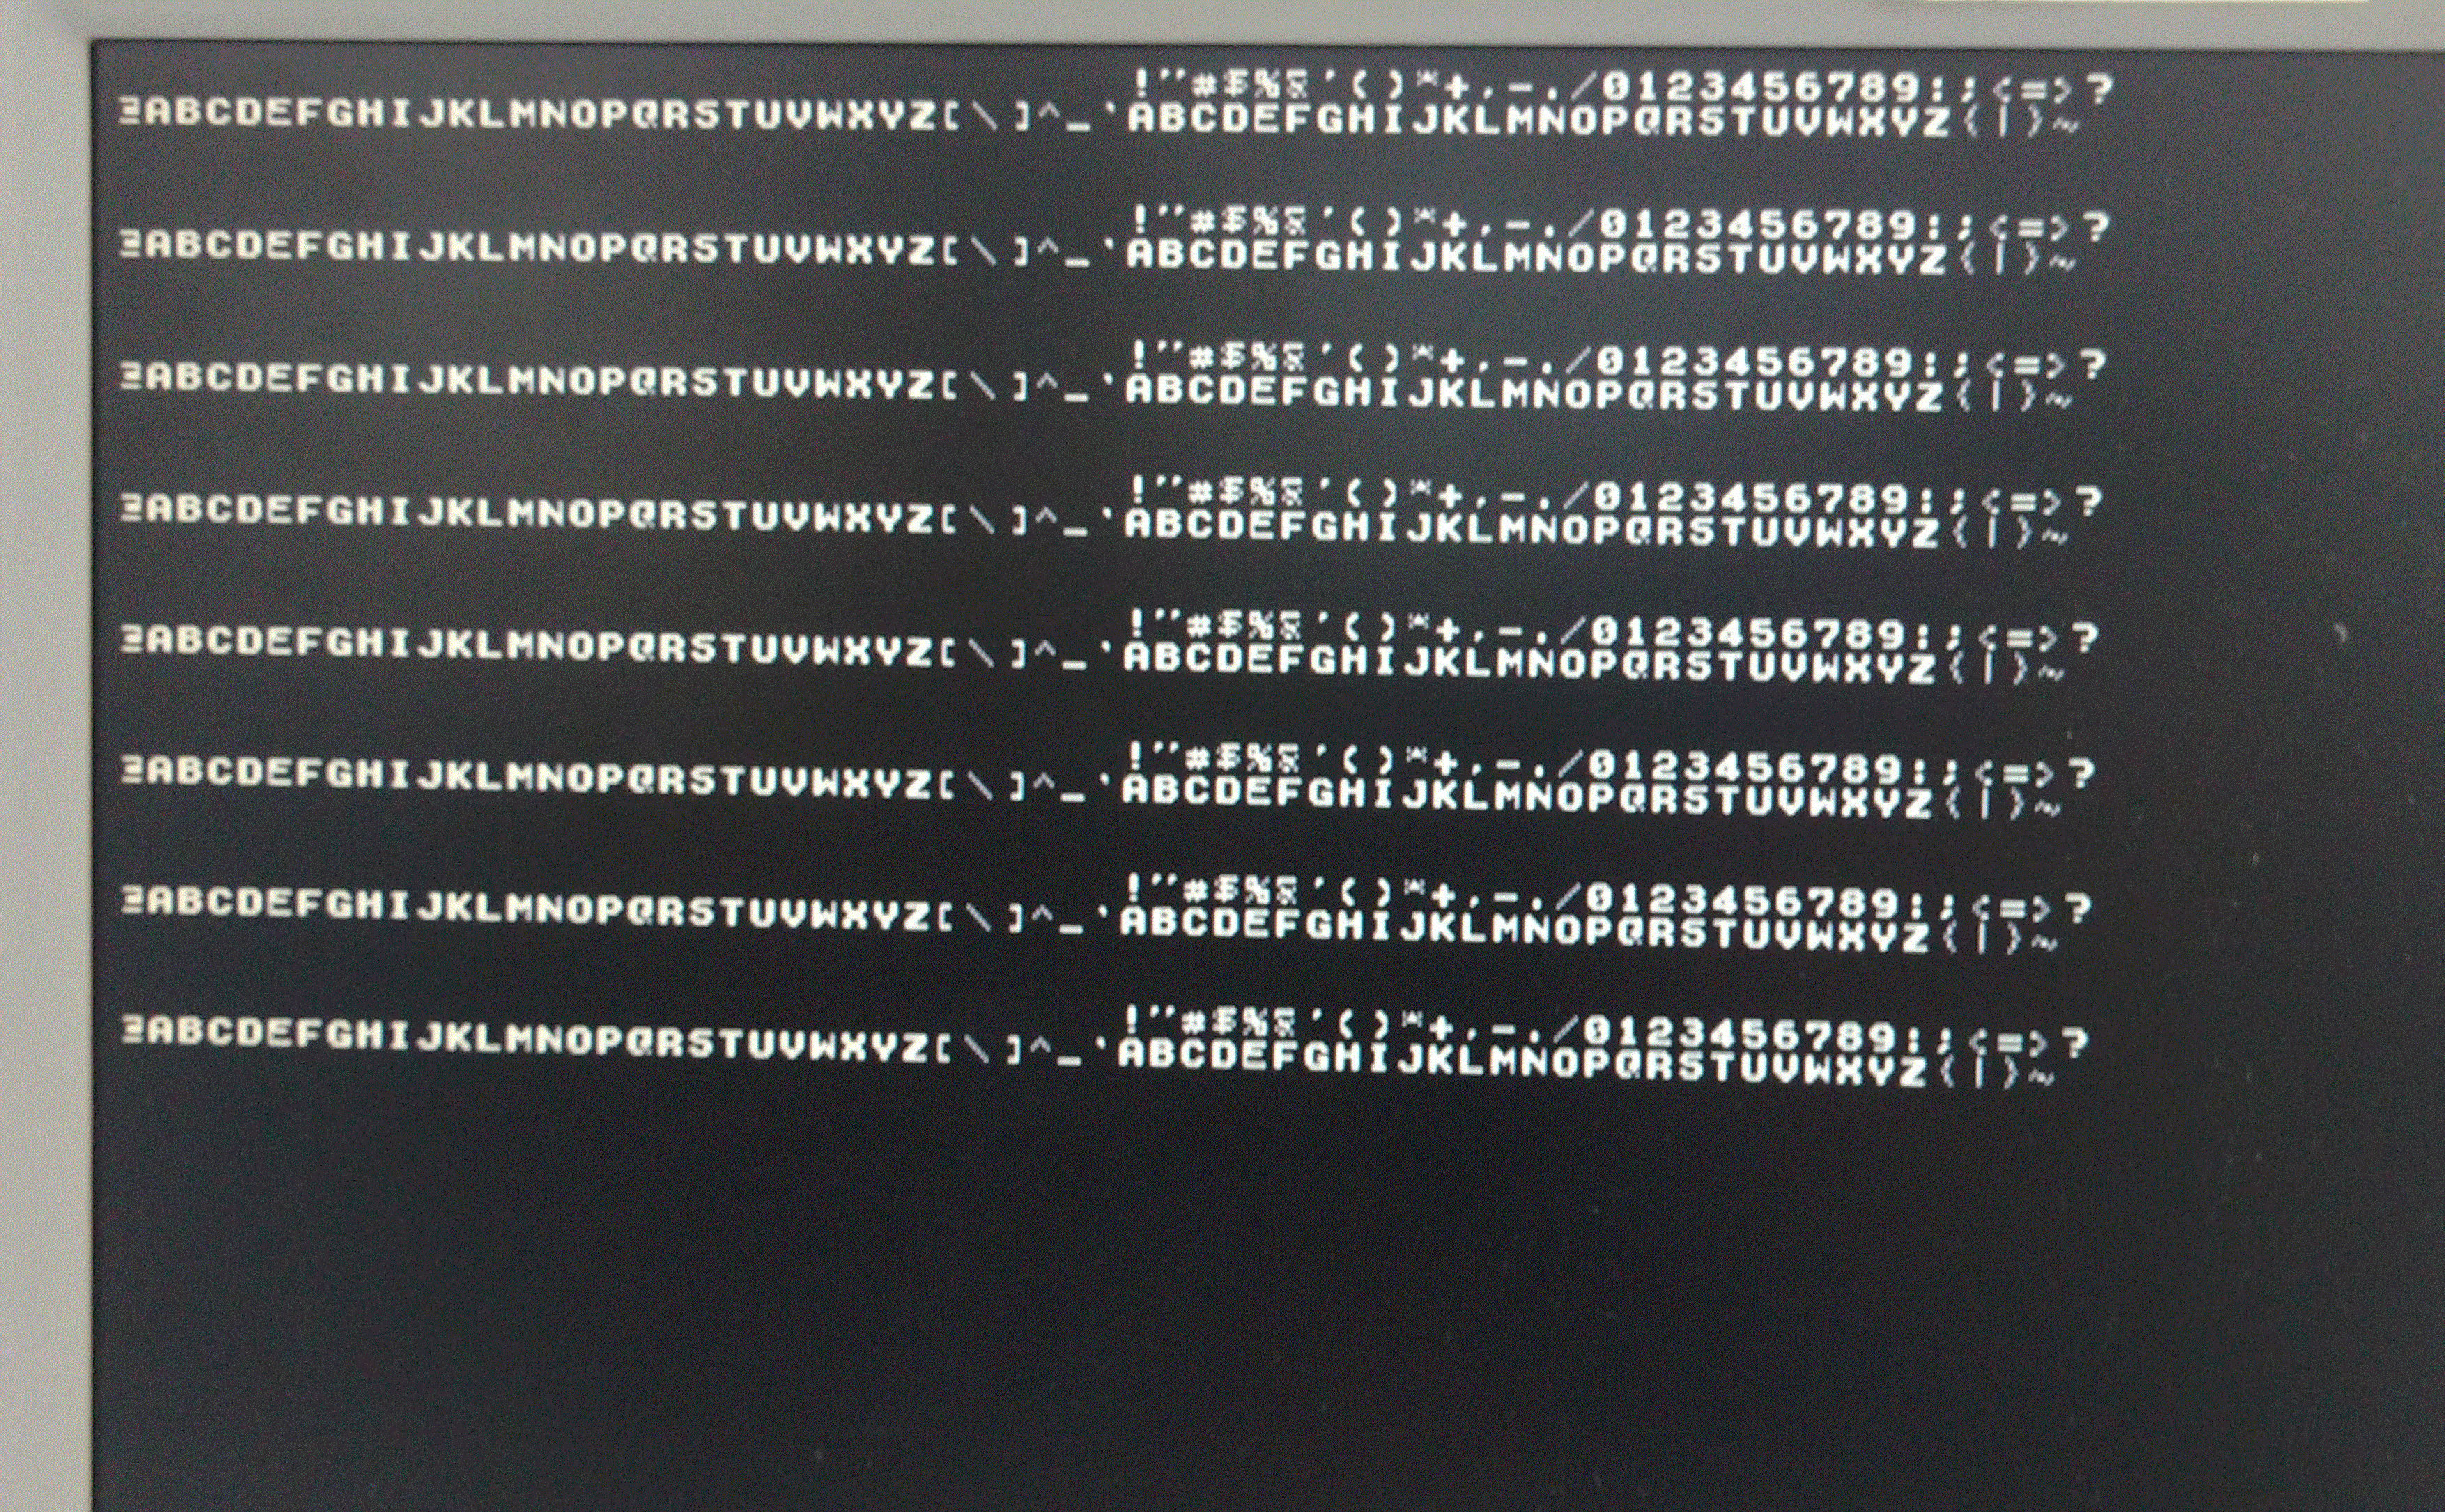
\includegraphics[width=0.7\textwidth]{asciiunitexample.png}
	\caption[Beispiel f\"ur die Textausgabe]{Beispiel f\"ur die Textausgabe: jedes darstellbare Zeichen wird abgebildet}
\end{figure}

\Section{\"Uberblick}

Die ASCII-Unit gibt auf dem Monitor, der \"uber die VGA-Schnittstelle des Entwicklungsboards angeschlossen wird, mittels Memory-Mapping den Inhalt des CHARRAM-Blocks in Form von ASCII-Zeichen wieder. Dazu wird jeweils eine Speicheradresse auf eine bestimmte Position auf dem Monitor (im Folgenden auch Zeichenplatz genannt) wie folgt abgebildet: Das Offset 0 repr\"astentiert das erste Zeichen (linkes oberes Eck), wobei mit jedem Schritt nach rechts das zugrundeliegende Offset inkrementell anw\"achst. Auf den letzten Buchstaben in einer Zeile folgt direkt der erste Buchstabe der darunter liegenden. So ergibt sich - analog zu einem zweidimensionalen Array - ein Zeilenumbruch nicht durch ein entsprechendes Steuerzeichen, sondern ist durch den Offset automatisch implizit gegeben. Es ergeben sich auf diese Weise 32 Zeilen mit je 64 Buchstaben, sodass insgesamt 2048 ASCII-Character gleichzeitig dargestellt werden k\"onnen. Die Basisadresse f\"ur den beschriebenen Speicherbereich stellt direkt die Basisadresse des CHARRAM-Blocks der MMU(\ref{ch:mmu}) dar.

Um ein Zeichen anhand seiner ASCII-Nummer darzustellen, wurde eine CHARMAP implementiert, die zu jedem der 256 ASCII Zeichen einen 64-Bit-Vektor bereitstellt hat. Dieser ist wiederum schlicht eine 8*8 Bitmap der Farbtiefe 1 BPP, sodass ein Character theoretisch den gesamten f\"ur ihn reservierten Bildschirmbereich erfassen kann. Allerdings  werden von diesen 64 Bit jeweils immer nur nur 6*6 tats\"achlich benutzt, woraus ein Zeilenabstand von 2 Pixeln resultiert. Diese im Bezug auf Ausnutzung des vorhandene Speicherplatzes zwar nicht optimale Umsetzung, erm\"oglichte allerdings eine einfache Implementierung: Positionelle Berechnungen, die unter anderem auf arithmetische Operationen wie Multiplikation und Division (welche aber nicht vom Rechenwerk \"ubernommen werden k\"onnen) zur\"uckgreifen, sind auf ganzzahligen Potenzen von 2 erheblich einfacher und weniger zeitintensiv zu realisieren.

\begin{figure}[H]
	\centering
		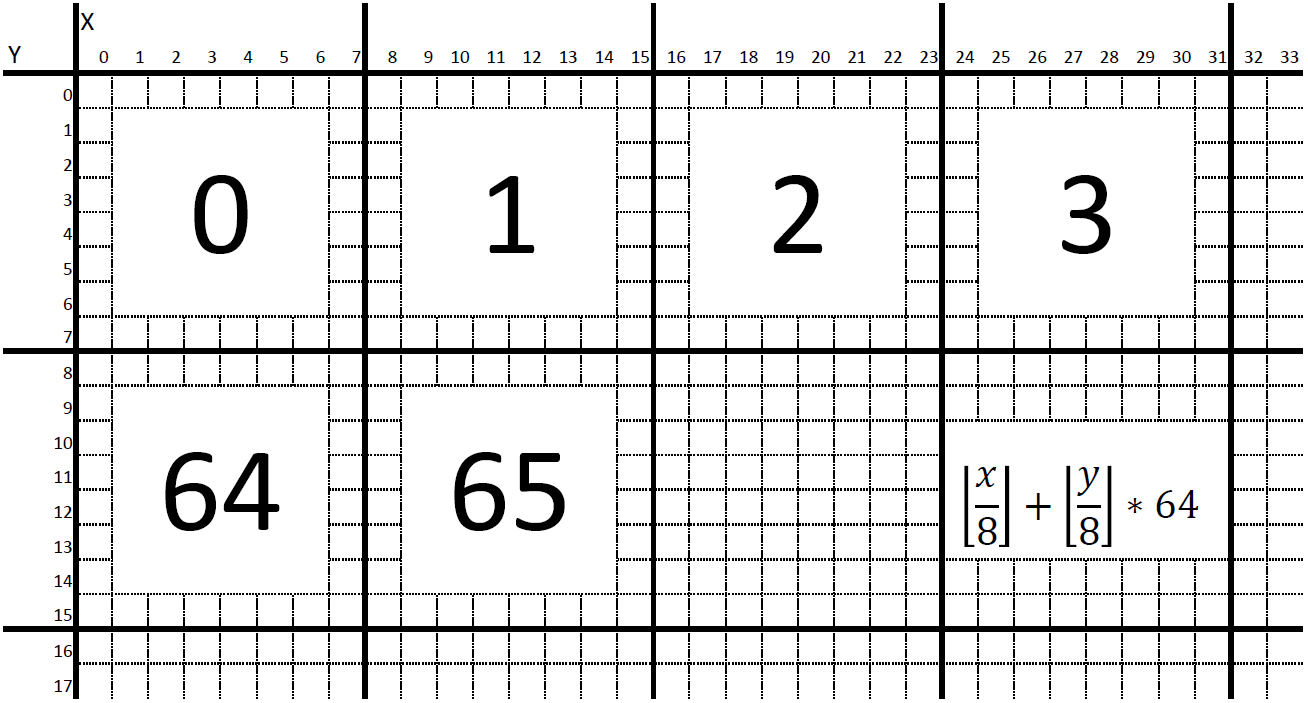
\includegraphics[width=1.0\textwidth]{Bildschirm.png}
	\caption[Veranschaulichung der Adressberechnung der ASCII-Unit]{Veranschaulichung der Adressberechnung anhand des Pixelfeldes des Monitors: Links oben wird von 0 ab nach rechts inkrementell iteriert. Die Adresse des Zeichenfeldes, das auf die Position (x,y) abbildet, errechnet sich wie folgt: $\lfloor \frac{x}{8} \rfloor + \lfloor \frac{y}{8} \rfloor * 64$. Das Bit f\"ur das aktuelle Pixel wird \"uber folgende Position aus dem 64-Bit-Vektor bestimmt: $(x\:  mod\:  8) + (y\:  mod\:  8) * 8$}
\end{figure}

Da eine Darstellung von Kleinbuchstaben innerhalb einer 6*6 Bitmap nur wenig Unterschied zur analogen Implementierung von Gro\ss{}buchstaben aufweist und eine Unterscheidung deshalb ohnehin nur schwerlich m\"oglich w\"are, greifen auch diese auf die Bitmaps der entsprechenden Gro\ss{}buchstaben zur\"uck. Aus der oben beschriebenen Implementierung geht direkt hervor, dass Steuerzeichen wie Tabulatoren oder Zeilenumbr\"uche keinerlei Effekt haben und deswegen auf leere Zeichen gemappt sind. Dies hat allerdings zur Folge, dass die Textformatierung durch entsprechende Software \"ubernommen werden muss.

Die ASCII-Unit wird, um die VGA-Schnittstelle ansprechen zu k\"onnen, wie diese ebenfalls mit 25 MHz getaktet. Dabei sendet die VGA-Unit mit jeder Taktflanke ein weiteres Pixel an das angeschlossene Ger\"at, wobei sich die Farbinformation dabei aufgrund der Farbtiefe von 1 BPP auf Schwarz/Wei\ss{} beschr\"ankt. Die Berechnung dieser Farbinformation erfolgt innerhalb der ASCII-Unit stufenweise mit einem resultierenden Pixel pro Taktflanke. 

\Section{Interface}
Neben dem bereits erw\"ahnten Takteingang gibt es jeweils einen Eingang f\"ur die x- und y-Koordinate des aktuellen Pixels (bzw. Position des Fadenstrahls) aus der VGA-Unit, welche mit jedem Takt aktualisiert werden und ein Ausgangssignal an die VGA-Einheit, welches angibt, ob das aktuelle Pixel gesetzt werden soll oder nicht.\\ Au{\ss}erdem gibt es zur Kommunikation mit dem CHARRAM in der MMU einen Ausgang, welcher die Adresse bzw. den Offset des Zeichenplatzes des aktuell zu berechnenden Pixels angibt sowie einen Eingang, der im darauffolgenden Takt die ASCII-Nummer des zugeh\"origen Zeichens erh\"alt.\\
Zur CHARMAP, die als ROM fungiert, wird der Takt durchgeleitet und ebenso die aus dem CHARRAM kommende ASCII-Nummer des aktuellen Zeichens, die hierbei als Adresse auftritt. Aus der CHARMAP kommt im darauffolgendem Takt der oben erw\"ahnte 64-Bit-Vektor der das jeweilige Zeichen repr\"asentiert.

\begin{figure}[H]
	\centering
	\label{fig:interface}
		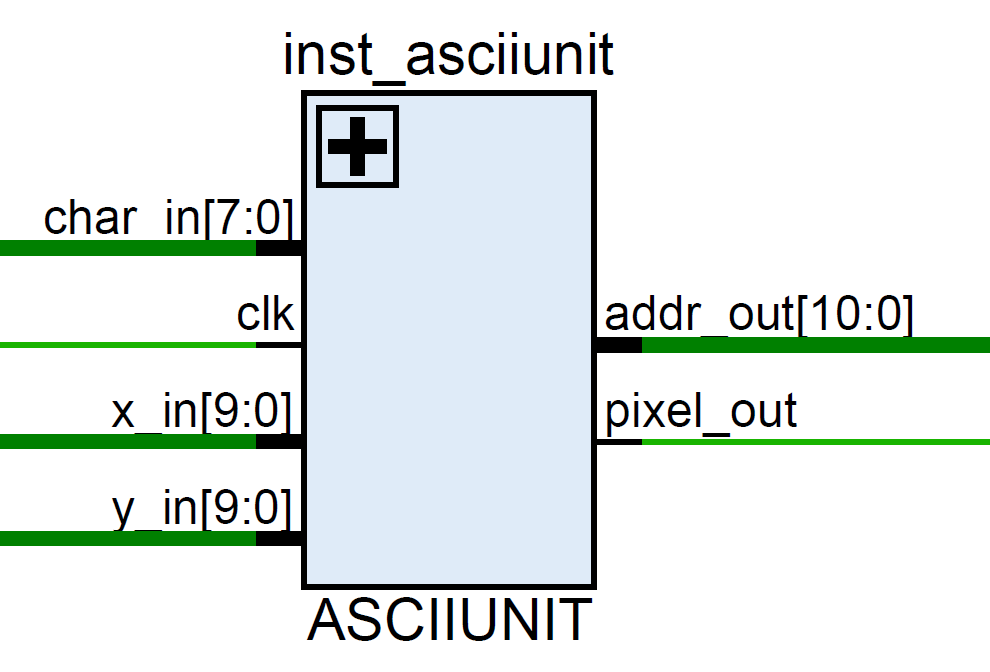
\includegraphics[width=0.3\textwidth]{Asciiunit.png}
	\caption[Interface der ASCII-Unit]{Das Interface der ASCII-Unit}
\end{figure}

\Section{Funktionsweise}

Da die stufenweise Berechnung der zu einer Position geh\"orenden Farbinformation mehr als einen Takt ben\"otigt, errechnet die ASCII-Unit diese bereits im Voraus: Dazu wird zun\"achst die Position des n\"achsten zu zeichnenden Bildschirmpixels eingelesen und die x-Koordinate um den Wert zwei inkrementiert.

Im darauf folgenden Takt wird aus der Positionsinformation der zugrundeliegende Offset innerhalb des CHARRAM-Blocks errechnet und an die MMU weitergeleitet. Dabei wird nicht das Zugriffsprotokoll, \"uber welches das Leitwerk mit der MMU kommuniziert, verwendet, sondern stattdessen erfolgt der Datenaustausch zwischen dem CHARRAM-Controller und der ASCII-Unit direkt durch weitergeleitete Signale innerhalb der MMU. Dies begr\"undet sich darin, dass die ASCII-Unit konstant mit Daten versorgt werden muss und ein regul\"arer Speicherzugriff dieser Anforderung nicht gen\"ugt. Der CHARRAM-Controller kann diesen gegebenenfalls zweiten lesenden Speicherzugriff insofern verarbeiten, dass der RAM-Block als Dual-Port-Blockram realisiert wurde. Ebenso spielt die asynchrone Taktfrequenz der MMU hierbei keinerlei entscheidende Rolle, da schlimmstenfalls derselbe Lesezugriff mehr als einen Takt anliegt, was aber die Valididt\"at der Daten keineswegs beeinflusst. Einzig schreibende Zugriffe der MMU auf die Speicherzelle, die zwischen den lesenden Zugriffen der ASCII-Unit auf dieselbe erfolgen, verursachen kurzweilige Probleme, da die in diesem Frame ausgegebenen Farbinformationen in diesem Fall nicht bzw. nur teilweise den gespeicherten Daten entsprechen. Allerdings h\"alt dieser fehlerhafte Zustand nur bis zum erneuten Zeichnen der entsprechenden Speicherposition an, sodass die fehlerhafte Darstellung mit blo\ss{}em Auge nicht zu erkennen ist.

Um im nächsten Takt anhand des ASCII-Codes einer Speicheradresse die der Position entsprechende Farbinformation innerhalb des derzeitigen Zeichens zu erhalten, wird die eingangs erw\"ahnte CHARMAP ausgelesen, indem der ASCII-Code aus der MMU direkt in die CHARMAP durchgeleitet wird. 

Dann wird die dazu erhaltene Bitmap entsprechend der Bildschirmposition ausgewertet. 

Zuletzt wird die resultierende Farbinformation dann an die VGA-Unit weitergeleitet, wobei im Hintergrund bereits, \"ahnlich einer Pipeline, die Verarbeitung der folgenden Pixel im Gange ist.

\begin{figure}[H]
	\centering
	\label{fig:overview}
		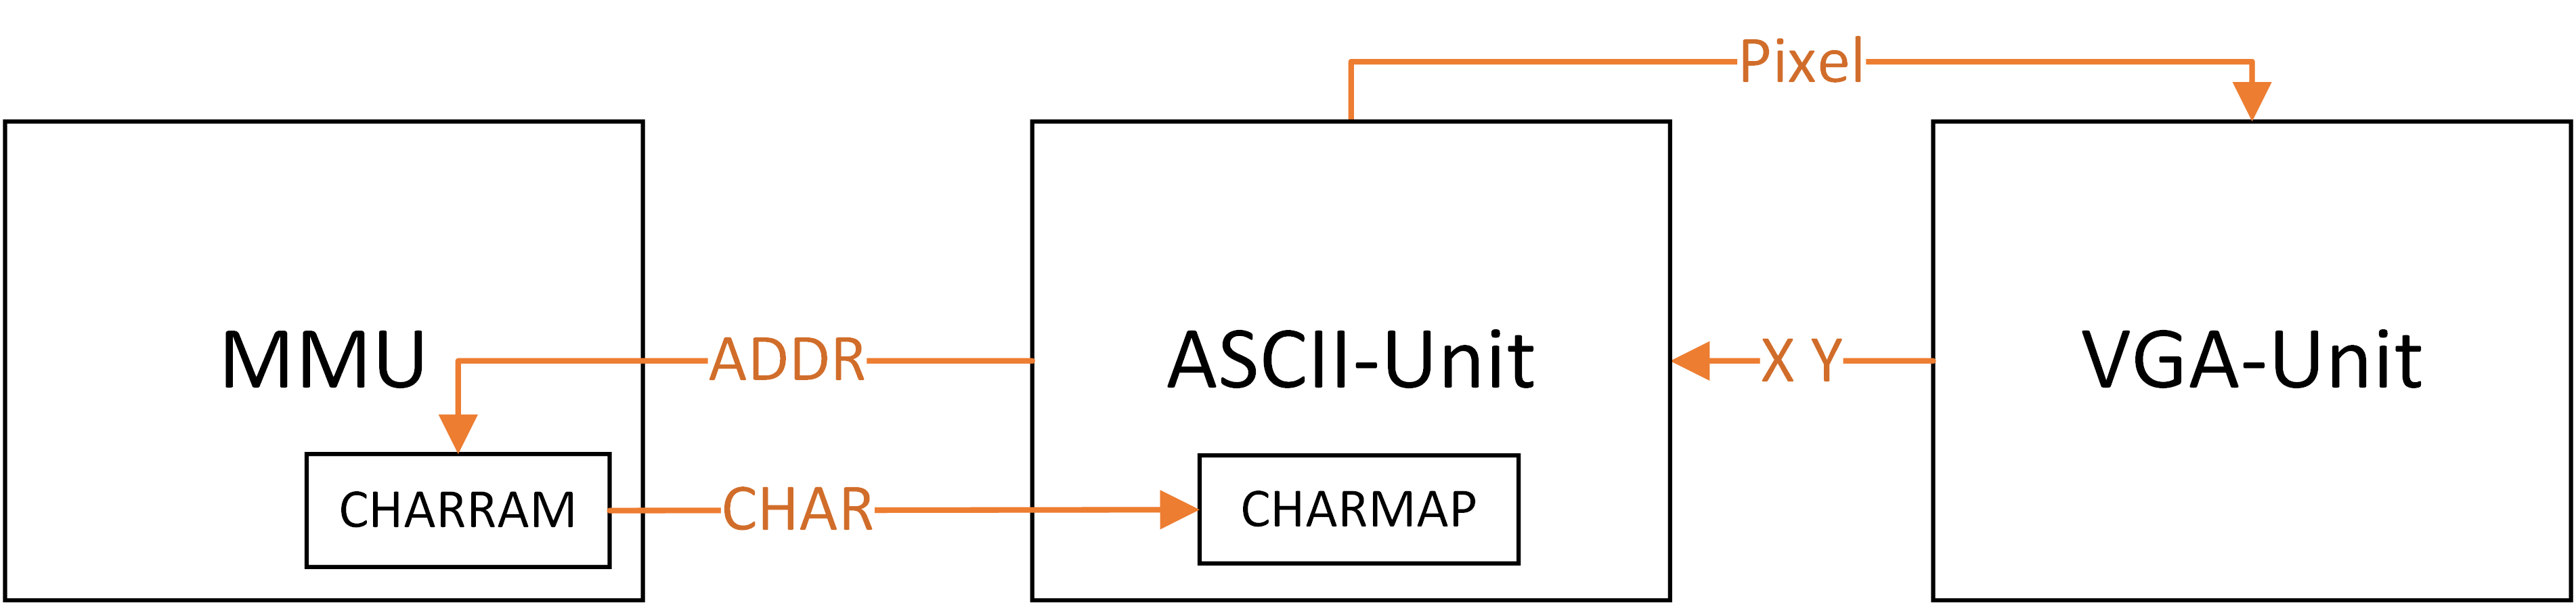
\includegraphics[width=1.0\textwidth]{ASCII.png}
	\caption[\"Ubersicht \"uber die ASCII-Unit]{\"Ubersicht: Beginn bei x- bzw. y-Koordinate; Verrechnung dieser zur Adresse f\"ur CHARRAM; dann Durchleiten in CHARMAP; anschlie\ss{}end Berechnung der Farbinformation; letztendlich Zur\"ucksenden an VGA-Unit}
\end{figure}

\newpage



\Chapter{Benutzerschnittstelle}

Im Folgenden wird die Benutzung des auf dem FPGA realisierten RISC-V Prozessors geschildert, wobei im Besonderen auf die Nutzerschnittstelle eingegangen wird. Um das FPGA in Betrieb zu nehmen, muss dieses logischerweise an eine entsprechende Stromquelle angeschlossen sein.

\Section{Initialisierung}

Im Allgemeinen kann ein Assemblerprogramm, das aus den implementierten Instruktionen zusammengesetzt ist, auf zwei Weisen in den Programmspeicher geladen und dann auf dem Prozessor ausgef\"uhrt werden.

\Subsection{Initialisierung durch BIOS und serielle Schnitstelle}

Die Programm-Einsprungsadresse, bei welcher die CPU die Ausf\"uhrung nach Beendigung eines Resets beginnt, Befehle abzuarbeiten, ist die erste Adresse des BIOS-RAM-Blocks \textit{0x00000000}. Dieser RAM-Block wird provisorisch mit einem einfachen BIOS-Programmcode initialisiert:


\begin{lstlisting}
	lui x1, 0x40000
	jalr x0, x1, 0
\end{lstlisting}

Dieser Programmcode f\"uhrt  die Ausf\"uhrung in einem anderen RAM-Block fort, dem SERIALRAM, welcher durch das Pr\"afix 0x4 auf die Speicheradresse \textit{0x40000000} gemappt ist. Der Programmierer muss zuvor also gew\"ahrleisten, dass dieser Speicherbereich, welcher durch die serielle Schnittstelle UART gef\"ullt wird, mit ausf\"uhrbarem Programmcode initialisiert wurde.

Indem der Programmierer nach einem Reset den Programmstart bei oben erw\"ahnter Einsprungsadresse durch das Halten des entsprechenden Blockadesignals auf Switch 4 (siehe Abbildung \ref{fig:pinning}) verz\"ogert, bleibt Zeit w\"ahrenddessen \"uber die UART Schnittstelle den SERIALRAM-Speicherblock zu initialisieren. Indem das Signal auf Switch 4 wieder entfernt wird, beginnt der Programmablauf wie eingangs erw\"ahnt im BIOS-RAM.
Da die serielle Schnittstelle nur f\"ur begrenzte Datenmengen verl\"asslich und fehlerfrei funktioniert, k\"onnen keine gr\"o\ss{}eren Programme auf diese Weise ausgef\"uhrt werden.

\Subsection{Initialisierung durch initiales Beschreiben des BIOS-RAM Blocks}

Alternativ besteht auch die M\"oglichkeit, den BIOS-RAM Block direkt beim Beschreiben des FPGAs mit dem auszuf\"uhrenden Programmcode zu initialisieren. Da der BIOS-RAM-Block als Dual-Port-Blockram realisiert wurde, kann dies ohne zeitlichen Aufwand bei einem Reset erfolgen.

Das BIOS wird auf diese Weise zweckentfremdet und der SERIALRAM Block bleibt ungenutzt. Auch muss das FPGA zur Ausf\"uhrung eines anderen Programms jedes Mal neu beschrieben werden. Trotz der genannten Nachteile aber bleibt diese Methode vorerst die einzig verl\"assliche Vorgehensweise, auch gr\"o\ss{}ere Datenmengen auf das Board zu \"ubertragen. Sie findet beispielsweise im Fall des sp\"ater beschriebenen Demoprogramms Anwendung.

\Section{Der Reset}

Nachdem das FPGA mit entsprechender Methodik initialisiert wurde oder aber nachdem eine Programmausf\"uhrung terminiert hat, muss der Prozessor zur\"uckgesetzt werden. Dies geschieht durch das kurzzeitige Halten des Reset-Signals, welches auf den Hardware-Switch \textit{SW 0} (siehe Abbildung \ref{fig:pinning}) gemappt ist.

Zu beachten ist, dass der Reset nur im verlangsamten Ausf\"uhrungsmodus (5 Hz) verl\"asslich funktioniert. Ob ein Reset im schnellen Ausf\"uhrungsmodus (50 MHz) erfolgreich verl\"auft, ist nichtdeterministisch und daher auch nicht zu empfehlen.

\Section{Graphische Oberfl\"achen}

Im Allgemeinen existieren zwei Methoden die Programmausf\"uhrung graphisch darzustellen: Einerseits existiert der Debugging-Modus, in welchem die Werte aller verf\"ugbaren Register sowie des Programmz\"ahlers und des Instruktionsregisters ausgegeben werden. Andererseits wird gleichzeitig der Speicherbereich des CHARRAM-Blocks auf eine ASCII-Darstellung gemappt. Mittels des Hardware-Switches \textit{SW 2} (siehe Abbildung \ref{fig:pinning}) wird bestimmt, welcher der beiden Modi auf dem VGA-Ausgang ausgegeben wird. Dabei bedeutet ein Halten des Switches die Darstellung \"uber ASCII und ein Loslassen die direkte Ausgabe der Register innerhalb der CPU.

\Subsection{Debugging-Modus}

Der Debugging-Modus zeichnet die verf\"ugbaren 32 Register x0-x31 bitweise auf das VGA-Ausgabeger\"at. Dabei werden die Register farblich voneinander getrennt und zeilenweise fortlaufend durchnummeriert (pro Zeile vier Register). Gesetzte Balken entsprechen einem gesetzten Bit innerhalb des Registerwerts, wobei das \textit{least significant Bit} links, und das \textit{most significant Bit} rechts dargestellt wird.
Die beiden separat dargestellten Register sind der Programmz\"ahler (links) sowie das Instruktionsregister (rechts), ebenfalls bitweise abgebildet.

\begin{figure}[H]
	\centering
	\label{fig:debuggingui}
		
\includegraphics[width=0.4\textwidth]{debugui.png}
	\caption[VGA-Ausgabe im Debugging-Modus]{VGA-Ausgabe im Debugging-Modus: PC und IR liegen zentral}
\end{figure}

Da die VGA-Ausgabe mit 25 MHz getaktet wird, der Prozessor im schnellen Ausf\"uhrungsmodus dagegen den vielfachen Takt erh\"alt, wechseln die Registerwerte unter Umst\"anden schneller, als sie dargestellt werden k\"onnen, wodurch es zu signifikanten Darstellungsfehlern kommen kann. Der Debugging-Modus ist dementsprechend, wie der Name bereits suggeriert lediglich f\"ur Debugging-Zwecke im langsamen Ausf\"uhrungsmodus sinnvoll nutzbar.

\Subsection{ASCII-Modus}
Der ASCII-Modus stellt zeilenweise fortlaufend durchnummeriert die Werte der Speicherzellen innerhalb des CHAR\-RAM-Blocks als ASCII-Zeichen dar. Die genaue Abbildungsmethodik wird in Kapitel \ref{ch:asciiunit} n\"aher erl\"autert.

Um das Demo-Programm sinnvoll zu benutzten, wird dieser Ausf\"uhrungsmodus empfohlen, da er einerseits auch im schnellen Ausf\"uhrungsmodus aufgrund der Seltenheit von schreibenden Speicherzugriffen im entsprechenden CHAR\-RAM-Block konsistenter Daten anzeigt, und andererseits das Programm so konzipiert ist, dass das Tic-Tac-Toe Spiel die ASCII-Schnittstelle zur Benutzerinteraktion vorsieht.

\Section{Benutzereingabe}

Analog zur Ausgabe von Daten bietet der Prozessor auch eine M\"oglichkeit zur Dateneingabe durch den Benutzer. Wie in Kapitel \ref{sec:mmuio} genauer erl\"autert wird, sind alle Buttons, Switches und LEDs auf Speicherzellen gemappt. Ein Halten oder Loslassen der entsprechenden Komponente f\"uhrt zu einem Wechsel des Bits an entsprechender Speicheradresse.

Programmierer haben so die M\"oglichkeit Benutzereingaben abzufragen oder auf diese zu reagieren, m\"ussen das aber innerhalb ihrer Implementierung selbst tun, da keinerlei Interrupts oder dergleichen bereitgestellt werden.

\newpage


\Chapter{Entwicklung eines Demo-Programms}

Das folgende Kapitel erl\"autert die Struktur, Motivation und Vorgehensweise hinter dem zu demonstrativen Zwecken entwickelten, auf dem Prozessor lauff\"ahigen Tic-Tac-Toe Programms. Dieses vereint alle zentralen Funktionalit\"aten der Prozessor-Implementierung auf dem FPGA.

\Section{Struktur und Funktion des Demo-Programms}

Wie eingangs geschildert, bietet das entwickelte Demo-Programm die M\"oglichkeit, \"uber die Buttons des FPGAs gegeneinander Tic-Tac-Toe zu spielen. Dabei wird mittels der Buttons BTN 0 bis BTN 3 (siehe Kapitel \ref{sec:mmuio}) \"uber das Spielbrett navigiert. Dabei ist das Brett zyklisch angeordnet, sodass eine Linksbewegung des Steuerkreuzes an den linken Rand dieses an die rechte Brettseite man\"ovriert. Mittels des Buttons BTN 4 (siehe Kapitel \ref{sec:mmuio}) setzt der Zugspieler seine Markierung an der zuvor ausgew\"ahlten Position, sofern dies regelkonform ist. Das Spiel enth\"alt keinen internen Reset und muss daher \"uber einen Hard-Reset durch das FPGA erfolgen.

\begin{figure}[H]
	\centering
	\label{fig:gameplay}
		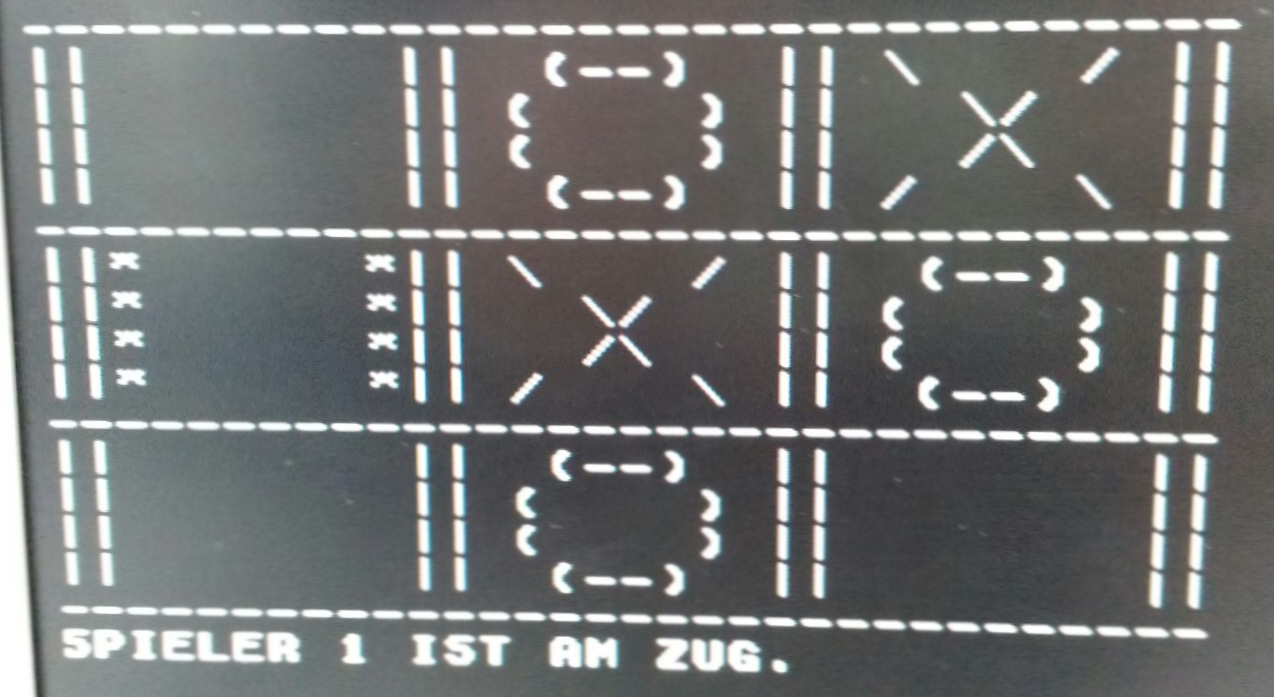
\includegraphics[width=0.6\textwidth]{gameplay.png}
	\caption{Bildschirmausgabe w\"ahrend der Ausf\"uhrung des Demo-Programms}
\end{figure}

Um m\"oglichst viel der implementierten Funktionalit\"at abzudecken, wurde bei der Implementierung darauf geachtet, die meisten Komponenten zu beanspruchen. So wird bei Programmstart im DDR2-SDRAM-Block eine, als Array von vorzeichenbehafteten 8-Bit Werten realisierte, Matrix $M$ wie folgt initialisiert:

\[ M = \begin{pmatrix} -4 & -4 & -4\\ -4 & -4 & -4\\ -4 & -4 & -4  \end{pmatrix}\;
 m_{i,j} = \begin{cases}
	0 & wenn\:Markierung\:von\:Spieler\:1 \\
	1 & wenn\:Markierung\:von\:Spieler\:2 \\
	-4 & sonst

\end{cases}\]

Wobei sich anhand dieser Definition durch Spalten-, Zeilen- und Diagonalsummen sofort der Zustand des Spiels ermitteln l\"asst: Ist diese gleich 0 oder 3, so hat einer der Kontrahenten das Spiel f\"ur sich entschieden.

Au\ss{}erdem werden die Komponenten der grafischen Oberfl\"ache mittels Schleifen und geeigneten Subroutinen im CHARRAM (siehe \ref{tab:ramlayout}) in ihren initialen Zustand versetzt. Dabei werden Sprungbefehle verwendet und auf diese Weise in die Demonstration miteinbezogen.

Da der Benutzer zwangsl\"aufig mit dem Board interagieren muss, um ein Spiel zu bestreiten, nutzt das Demo-Programm auch die zuvor beschriebenen Memory-Mapped-I/O Funktionalit\"aten aus. Dazu wird, wie im folgenden Ausschnitt des Programmcodes gezeigt, in einer Endlosschleife nach neuen Eingaben auf den f\"unf verwendeten Buttons gesucht, indem durch Puffern des letzten Zustands und bitweise Verkn\"upfungen des gerade losgelassenen Buttons ermittelt wird und die Button-Nummer als R\"uckgabewert liefert. Nebeneffekte des Prellens werden hierbei allerdings nicht ber\"ucksichtigt.

\begin{lstlisting}
.key_release
	lui x26, 0x30000 //ioram prefix
	lh x27, x26, 0
	srli x27, x27, 7
	andi x27, x27, 0x1F //isolating buttons
	.key_release_wait
		//load new keys and check if any key was released
		lh x28, x26, 0
		srli x28, x28, 7
		andi x28, x28, 0x1F //new key input
		addi x30, x28, 0
		xor x28, x28, x27 //event vector (pressed and released keys)
		and x28, x28, x27 //filter released keys
		addi x27, x30, 0
		beq x28, x0, key_release_wait //keep waiting
	addi x18, x0, 0 //return value := which button was pressed
	addi x29, x0, 1
	.key_release_shift_result
		beq x28, x29, end_key_release
		srli x28, x28, 1
		addi x18, x18, 1
		jal x0, key_release_shift_result
	.end_key_release
	jalr x0, x1, 0
\end{lstlisting}

Der gesamte Programmcode umfasst circa 400 Zeilen und liegt der VHDL-Implementierung bei, wurde aber aufgrund des unverh\"altnissm\"a\ss{}igen Umfangs an dieser Stelle ausgelassen und durch den obigen Ausschnitt repr\"asentativ ersetzt.

\Section{Assemblierer und Simulator}

Aufgrund der eben erw\"ahnten Programmgr\"o\ss{}e, des reduzierten Instruction Sets und der projektspezifischen RAM-Struktur wurde der Beschluss gefasst, beim Assemblieren des Programmcodes auf einen im Rahmen des Projekts programmierten Assemblierer zur\"uckzugreifen. Auch das Debugging erfolgte durch ein eigenes Tool, welches beispielsweise Aspekte des Memory-Mapped-I/O ber\"ucksichtigen und entsprechend simulieren kann. Die beiden Programme wurden in der Skriptsprache Python entwickelt und gen\"ugen den Anspr\"uchen des Projekts insofern, als dass ein Assemblerprogramm entsprechend assembliert und simuliert werden kann, die Software allerdings keineswegs ausgiebig auf Stabilit\"at oder dergleichen getestet wurde, zumal dies nicht als Schwerpunkt f\"ur das Projekt gesetzt war.

\Subsection{Assemblierer}

Der Assemblierer ist dabei in der Lage aus einem Eingabeprogrammcode, welches Spr\"unge, Labels und Kommentare enthalten kann, einerseits Bytecode sowie eine Symboltabelle zu erstellen. Des Weiteren wird der assemblierte Programmcode auch in korrekter VHDL-Syntax ausgegeben, sodass dieser zur Initialisierung einer Dual-Port-Blockram Komponente direkt eingebunden werden kann. Dabei wird der Assemblierer als Python-Script mit den Eingabewerten als Parametern aufgerufen:

\begin{lstlisting}[language=bash]
   $ python riscv_as.py -i {input} -o {output(vhdl)} -s {symbols} -b {binary}
\end{lstlisting}

Die Symboltabelle gibt dabei Auskunft \"uber die Speicheradresse eines im Programmcode definierten Labels. Aufgrund des modularen Aufbaus des Assemblierers k\"onnen Erweiterungen des Befehlssatzes sowie andere syntaktische Feinheiten dem Parsing- und Compilingprozess problemlos hinzugef\"ugt werden.

\Subsection{Simulator}
 
Der Simulator ist als Backend-Erweiterung zum Assemblierer gedacht, da dieser mithilfe der Ausgabedateien den Programmablauf simulieren kann. Analog zu bekannten Debugging-Umgebungen unterst\"utzt der Simulator das Setzen von Breakpoints sowie das Schrittweise Ausf\"uhren eines Befehls, w\"ahrend die verf\"ugbaren Register direkt im Blick behalten werden k\"onnen. Ferner ist es aber auch m\"oglich, den Programmablauf nach einem bestimmten Zeitintervall automatisch zu unterbrechen oder aber bestimmte Eingabesignale zu stimulieren (auch hier kann mit einem beliebigen Zeitintervall gearbeitet werden). Das Python-Script des Simulators wird in Verbindung mit dem Assemblierer wie folgt aufgerufen:

\begin{lstlisting}
   $ python riscv_as.py -i {input} -o {output(vhdl)} -s {symbols} -b {binary}
   $ python riscv_simulation.py -s {symbols} -b {binary}
\end{lstlisting}

Dabei startet der Simulator an der Programmeinsprungsadresse und unterst\"utzt die folgenden Befehle:

\begin{table}[h]
\begin{center}
	\begin{tabular}{| l | l |}
	\hline
		\textbf{Befehl} & \textbf{Beschreibung} \\ \hline
		n & F\"uhrt n\"achsten Befehl aus \\ \hline
		s & F\"uhrt Subroutine aus, ohne in diese zu springen\\ \hline
		c & Setzt Programmausf\"uhrung fort \\ \hline
		printchars & Zeigt die Ausgabe der ASCII-Unit\\ \hline
		bp {label/offset} & Neuer Breakpoint\\ \hline
		pin show & Zeigt alle I/O-Signale\\ \hline
		pin set {pinid} {0/1} [-d duration] & Setzt ein I/O-Signal auf einen Wert (ggf. f\"ur ein Zeitintervall in s)\\ \hline
		 m {offset} {cnt} [chunksize] & Stellt die Speicherzellen eines bestimmten Offsets blockweise dar\\ \hline
		 sleep {duration} & Unterbricht die Programmausf\"uhrung nach einem Zeitintervall in s\\ \hline 
	\end{tabular}
\end{center}
\caption{Befehls\"ubersicht des Simulators}
\end{table}

Dabei wird durch die eben beschriebenen Befehle durch die Programmausf\"uhrung navigiert, um so potenzielle Fehlerquellen zu entdecken und berichtigen. Zur Entwicklung des Demo-Programms hat der Simulator eine ma\ss{}gebliche Rolle gespielt: Nur dank dessen Funktionalit\"aten war es \"uberhaupt m\"oglich, mit vertrebarem Aufwand ein vergleichsweise komplexes, funktionst\"uchtiges Programm zu entwerfen.


\appendix{}
\Chapter{Anhang}
\documentclass{standalone}

\usepackage{style}
\usepackage{tikz}
\usetikzlibrary{arrows}

\begin{document}
\begin{tikzpicture}[>=triangle 45]
\draw[line width=3pt] (0,0) rectangle node {ALU} (18,3);
\draw[->] (1.5,-3) node[below] {\Vhdl{alu\_data\_out1}} -- (1.5,0) node[above] {\Vhdl{cu\_data\_in1}};
\draw[->] (4.5,-3) node[below] {\Vhdl{alu\_data\_out2}} -- (4.5,0) node[above] {\Vhdl{cu\_data\_in2}};
\draw[->] (7.5,-3) node[below] {\Vhdl{alu\_adr\_out}} -- (7.5,0) node[above] {\Vhdl{cu\_adr\_in}};
\draw[->] (10.5,-3) node[below] {\Vhdl{alu\_com\_out}} -- (10.5,0) node[above] {\Vhdl{cu\_com\_in}};
\draw[->] (13.5,-3) node[below] {\Vhdl{alu\_work\_out}} -- (13.5,0) node[above] {\Vhdl{cu\_work\_in}};
\draw[<-] (16.5,-3) node[below] {\Vhdl{alu\_data\_in}} -- (16.5,0) node[above] {\Vhdl{cu\_data\_out}};
\draw[line width=3pt] (0,-3) rectangle node {Leitwerk} (18,-6);
\draw[<-] (1.5,-9) node[below] {\Vhdl{data\_in}} -- (1.5,-6) node[above] {\Vhdl{mmu\_data\_out}};
\draw[<-] (4.5,-9) node[below] {\Vhdl{addr\_in}} -- (4.5,-6) node[above] {\Vhdl{mmu\_adr\_out}};
\draw[<-] (7.5,-9) node[below] {\Vhdl{cmd\_in}} -- (7.5,-6) node[above] {\Vhdl{mmu\_com\_out}};
\draw[<-] (10.5,-9) node[below] {\Vhdl{work\_in}} -- (10.5,-6) node[above] {\Vhdl{mmu\_work\_out}};
\draw[->] (13.5,-9) node[below] {\Vhdl{data\_out}} -- (13.5,-6) node[above] {\Vhdl{mmu\_data\_in}};
\draw[->] (16.5,-9) node[below] {\Vhdl{ack\_out}} -- (16.5,-6) node[above] {\Vhdl{mmu\_ack\_in}};
\draw[line width=3pt] (0,-9) rectangle node {MMU} (18,-12);
\end{tikzpicture}
\end{document}


\clearpage{}
\Section{Known Bugs}
\begin{description}
\item[ASCII-Ausgabe] Teile des Zeichens an Position 0 werden in den
darunterliegenden Zeilen ebenfalls angezeigt.
\item[Leitwerk, MMU] Beim LOAD-Befehl sollte die MMU lediglich die ben\"otigte
Anzahl an Bits laden und nicht immer 32 Bits.
\item[Leitwerk,MMU] Der Prozessor st\"urtzt, vermutlich wegen
Synchronisationsfehlern zwischen Leitwerk und MMU, gelegentlich ab. Au\ss{}erdem f\"uhrt ein Reset im schnellen Modus dadurch gelegentlich ebenfalls zu Inkonsistenzen und Programmabst\"urzen.
\item[ALU] Die ALU wartet wahrscheinlich l\"anger auf das Ergebnis der
Divisionseinheit, als n\"otig w\"are.
\item[MMU] Durch eine Unterscheidung der Speicherarten bei Speicherzugriffen
k\"onnte man hier eine Geschwindigkeitssteigerung erzielen.
\item[Leitwerk] Das Leitwerk wartet am Ende einiger Befehle noch 3 Takte auf
die ALU, ohne dass diese vorher gestartet wurde.
\item[MMU, allgemein] Die Buttons und Switches werden nicht entprellt.
\item[UART] Die UART-Einheit korrigiert keine Fehler in der \"Ubertragung,
weshalb nur eine sehr begrenzte Datenmenge fehlerfrei \"ubertragen werden kann.
Dadurch k\"onnen bei einer Programmierung durch die serielle Schnittstelle nur
sehr kleine Programme zum Einsatz kommen.
\item[UART] Die serielle Schnittstelle kann w\"ahrend der normalen
Codeausf\"uhrung des Prozessors nicht zuverl\"assig genutzt werden, da die
Refresh-Zyklen des DDR2-RAMs die Befehlsausf\"uhrung behindern und dadurch
\"ubertragene Bytes verpasst werden.
\item[allgemein] Ein Reset ist nur im langsamen Modus zuverl\"assig m\"oglich. Im
schnellen Modus kann eine Reset zum Absturz des Prozessors f\"uhren.
\end{description}

\clearpage{}
\Section{Ausf\"uhrungsdauer der Befehle}

\begin{table}[H]
\begin{minipage}[t]{.5\textwidth}
\centering
\begin{tabular}{|l|l|l|l|}
\hline
Befehl(e)          & \multicolumn{3}{l|}{Ausf\"uhrungsdauer (in Takten)} \\
\hline
                   & \(s\leq{}2\) & \(2<s<4\)    & \(s\geq{}4\)           \\
\hline
\Instr{LUI}        & \(4\)        & \(4\)        & \(s\)                  \\
\Instr{AUPIC}      & \(4\)        & \(4\)        & \(s\)                  \\
\Instr{JAL}        & \(8\)        & \(8\)        & \(4+s\)                \\
\Instr{JALR}       & \(8\)        & \(8\)        & \(4+s\)                \\
\Instr{BEQ}        & \(12\)       & \(12\)       & \(8+s\)                \\
\Instr{BNE}        & \(12\)       & \(12\)       & \(8+s\)                \\
\Instr{BLT}        & \(12\)       & \(12\)       & \(8+s\)                \\
\Instr{BLTU}       & \(12\)       & \(12\)       & \(8+s\)                \\
\Instr{BGE}        & \(12\)       & \(12\)       & \(8+s\)                \\
\Instr{BGEU}       & \(12\)       & \(12\)       & \(8+s\)                \\
\Instr{LB}         & \(10\)       & \(8+s\)      & \(4+2\cdot{}s\)        \\
\Instr{LBU}        & \(10\)       & \(8+s\)      & \(4+2\cdot{}s\)        \\
\Instr{LH}         & \(10\)       & \(8+s\)      & \(4+2\cdot{}s\)        \\
\Instr{LHU}        & \(10\)       & \(8+s\)      & \(4+2\cdot{}s\)        \\
\Instr{LW}         & \(10\)       & \(8+s\)      & \(4+2\cdot{}s\)        \\
\Instr{SB}         & \(13\)       & \(11+s\)     & \(8+2\cdot{}s\)        \\
\Instr{SH}         & \(13\)       & \(11+s\)     & \(8+2\cdot{}s\)        \\
\Instr{SW}         & \(13\)       & \(11+s\)     & \(8+2\cdot{}s\)        \\
\Instr{ADDI}       & \(4\)        & \(4\)        & \(s\)                  \\
\Instr{SLTI}       & \(4\)        & \(4\)        & \(s\)                  \\
\Instr{SLTIU}      & \(4\)        & \(4\)        & \(s\)                  \\
\Instr{XORI}       & \(4\)        & \(4\)        & \(s\)                  \\
\Instr{ORI}        & \(4\)        & \(4\)        & \(s\)                  \\
\Instr{ANDI}       & \(4\)        & \(4\)        & \(s\)                  \\
\Instr{SLLI}       & \(4\)        & \(4\)        & \(s\)                  \\
\Instr{SRLI}       & \(4\)        & \(4\)        & \(s\)                  \\
\Instr{SRAI}       & \(4\)        & \(4\)        & \(s\)                  \\
                   &              &              &                        \\
\hline
\end{tabular}
\end{minipage}%
\begin{minipage}[t]{.5\textwidth}
\centering
\begin{tabular}{|l|l|l|l|}
\hline
Befehl(e)          & \multicolumn{3}{l|}{Ausf\"uhrungsdauer (in Takten)} \\
\hline
                   & \(s\leq{}2\) & \(2<s<4\)    & \(s\geq{}4\)           \\
\hline
\Instr{ADD}        & \(4\)        & \(4\)        & \(s\)                  \\
\Instr{SUB}        & \(4\)        & \(4\)        & \(s\)                  \\
\Instr{SLL}        & \(4\)        & \(4\)        & \(s\)                  \\
\Instr{SLT}        & \(4\)        & \(4\)        & \(s\)                  \\
\Instr{SLTU}       & \(4\)        & \(4\)        & \(s\)                  \\
\Instr{XOR}        & \(4\)        & \(4\)        & \(s\)                  \\
\Instr{SRL}        & \(4\)        & \(4\)        & \(s\)                  \\
\Instr{SRA}        & \(4\)        & \(4\)        & \(s\)                  \\
\Instr{OR}         & \(4\)        & \(4\)        & \(s\)                  \\
\Instr{AND}        & \(4\)        & \(4\)        & \(s\)                  \\
\Instr{FENCE}      & -            & -            & -                      \\
\Instr{FENCE.I}    & -            & -            & -                      \\
\Instr{SCALL}      & -            & -            & -                      \\
\Instr{SBREAK}     & -            & -            & -                      \\
\Instr{RDCYCLE}    & \(4\)        & \(4\)        & \(s\)                  \\
\Instr{RDCYCLEH}   & \(4\)        & \(4\)        & \(s\)                  \\
\Instr{RDTIME}     & \(4\)        & \(4\)        & \(s\)                  \\
\Instr{RDTIMEH}    & \(4\)        & \(4\)        & \(s\)                  \\
\Instr{RDINSTRET}  & \(4\)        & \(4\)        & \(s\)                  \\
\Instr{RDINSTRETH} & \(4\)        & \(4\)        & \(s\)                  \\
\Instr{MUL}        & \(4\)        & \(4\)        & \(s\)                  \\
\Instr{MULH}       & \(4\)        & \(4\)        & \(s\)                  \\
\Instr{MULHSU}     & \(4\)        & \(4\)        & \(s\)                  \\
\Instr{MULHU}      & \(4\)        & \(4\)        & \(s\)                  \\
\Instr{DIV}        & \(35\)       & \(35\)       & \(max(s,35)\)          \\
\Instr{DIVU}       & \(35\)       & \(35\)       & \(max(s,35)\)          \\
\Instr{REM}        & \(35\)       & \(35\)       & \(max(s,35)\)           \\
\Instr{REMU}       & \(35\)       & \(35\)       & \(max(s,35)\)           \\
\hline
\end{tabular}
\end{minipage}
\caption[\"Ubersicht \"uber die Ausf\"uhrungsdauer der Befehle]{\"Ubersicht 
\"uber die Ausf\"uhrungsdauer der Befehle. Da die Dauer eines Speicherzugriffs abh\"angig von dem angesprochenen Speichertyp und selbst dann nicht immer
exakt vorhersagbar ist, werden hier f\"ur unterschiedliche
Speicherzugriffsdauern \(s\) die jeweilige Ausf\"uhrungsdauer der Befehle
gelistet.}
\end{table}

\clearpage{}
\Section{1. Pflichtenheft vom 02.06.2016}

\begin{figure}[H]
\centering
\frame{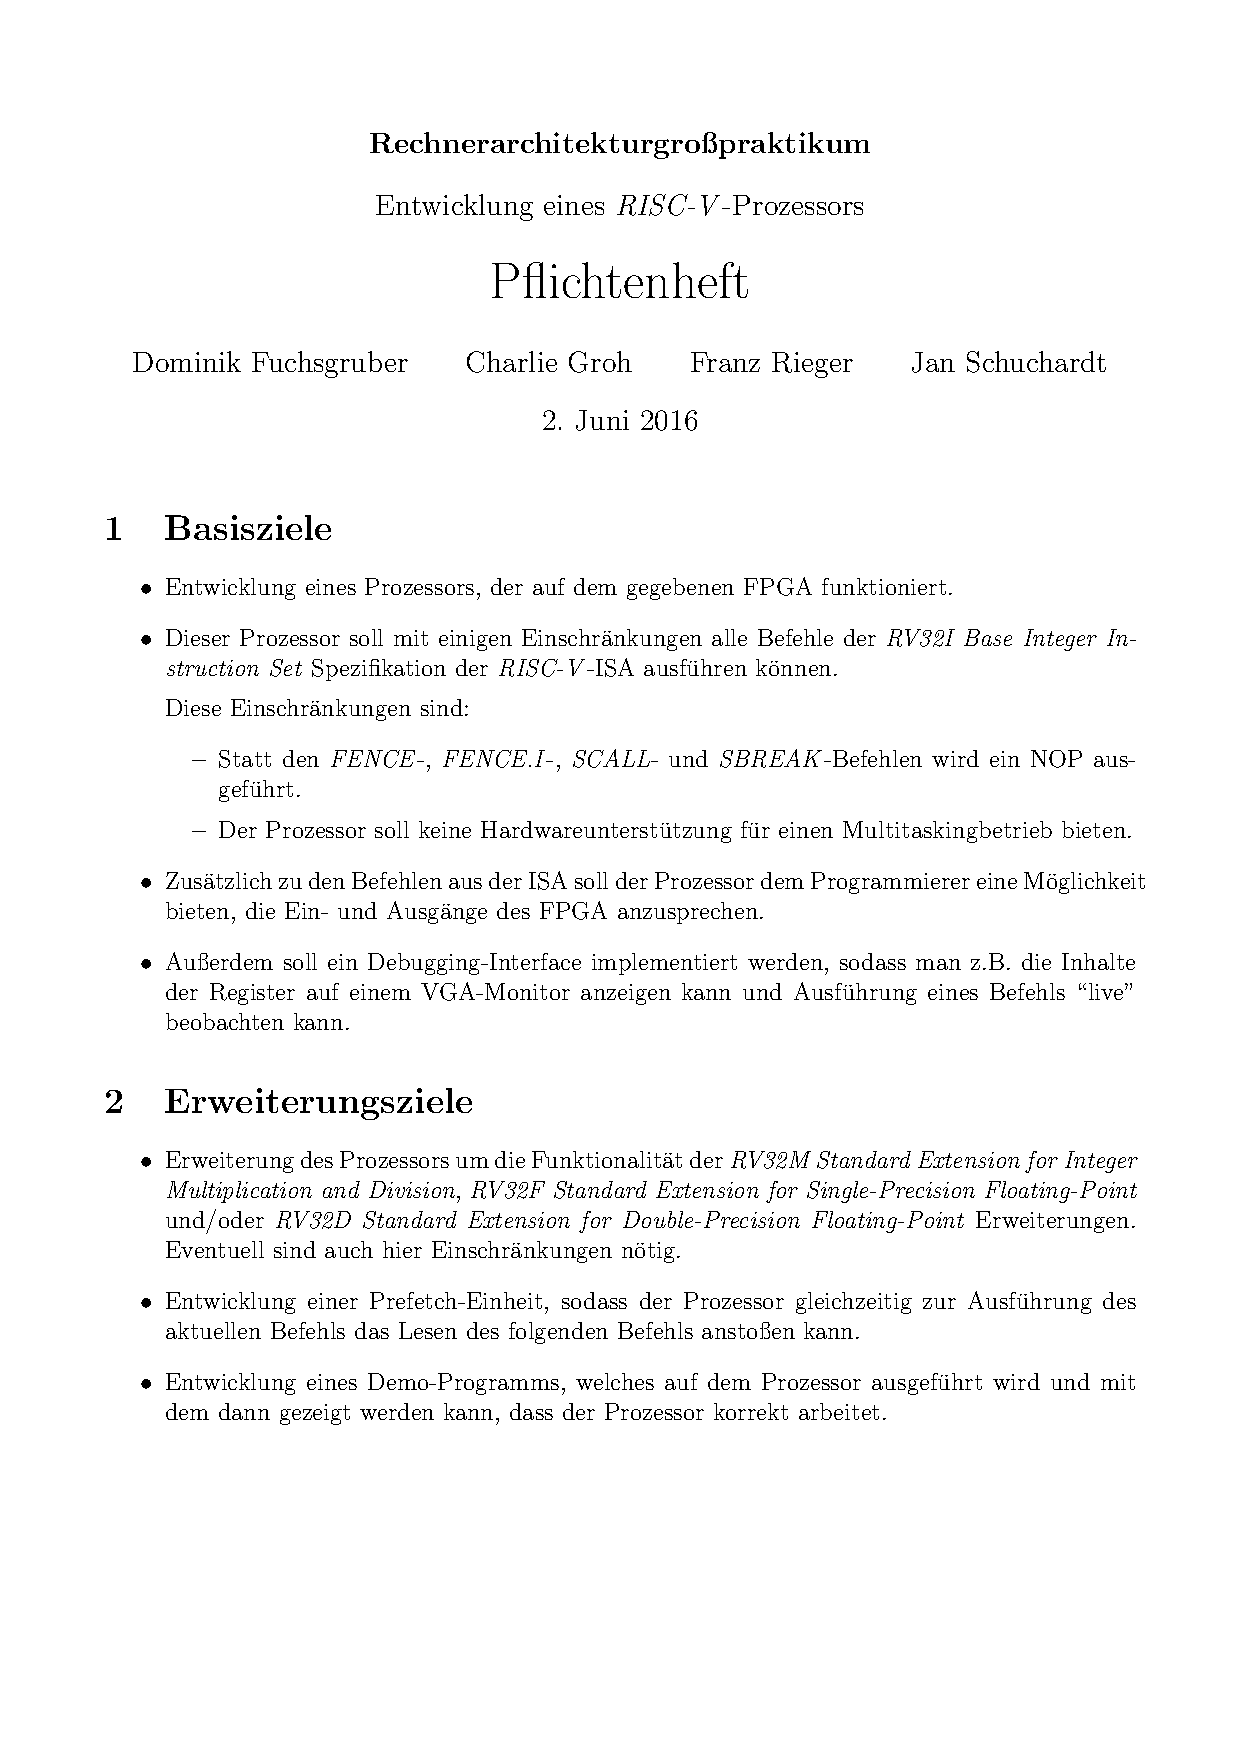
\includegraphics[scale=0.64]{./appendix/img/pflichtenheft1.pdf}}
\caption[Pflichtenheft vom 02.06.2016]{Pflichtenheft vom 02.06.2016}
\end{figure}

\clearpage{}
\Section{2. Pflichtenheft vom 19.11.2016}

\begin{figure}[H]
\centering
\frame{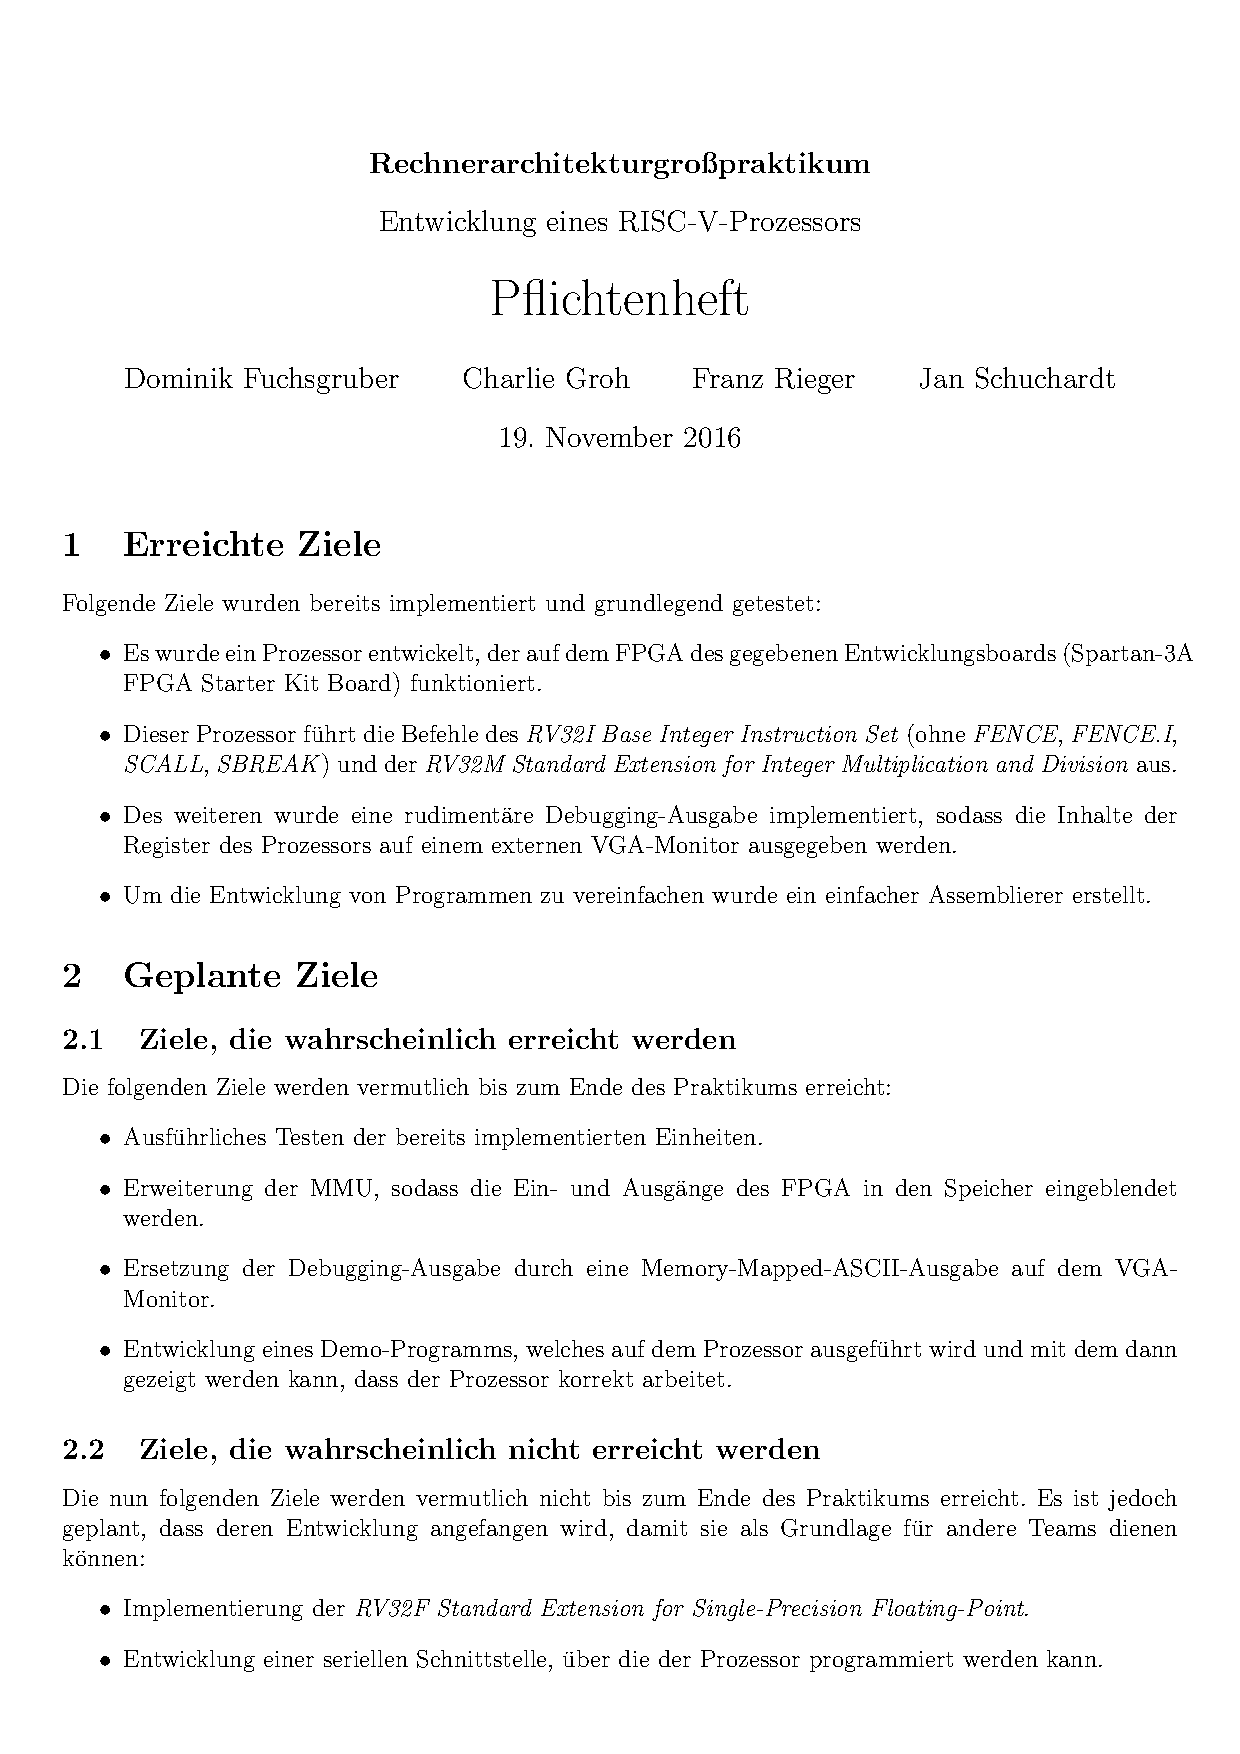
\includegraphics[scale=0.64]{./appendix/img/pflichtenheft2.pdf}}
\caption[Pflichtenheft vom 19.11.2016]{Pflichtenheft vom 19.11.2016}
\end{figure}

\clearpage{}
\end{document}
\end{tabluar}
